\newpage
\section{TCGAbiolinksGUI: A graphical user interface to analyze GDC cancer molecular and clinical data}

Although TCGAbiolinks is a suitable R package for most data analysts with a strong knowledge and familiarity with R specifically those who can comfortably write R commands, we developed TCGAbiolinksGUI to enable user access to the methodologies offered in TCGAbiolinks and to give users the flexibility of point-and-click style analysis without the need to enter specific arguments. TCGAbiolinksGUI takes in all the important features of TCGAbiolinks and offers a graphics user interface (GUI) thereby eliminating any need to familiarize TCGAbiolinks' key functions and arguments.

\subsection{Infrastructure}
The TCGAbiolinksGUI user interface was created using Shiny, a Web Application Framework for R, and uses several packages to provide advanced features that can enhance Shiny apps, such as shinyjs to add JavaScript actions \cite{shinyjs}, shinydashboard to add dashboards \cite{shinydashboard} and shinyFiles \cite{shinyFiles} to provide access to the server file system.

The following R/Bioconductor packages are used as back-ends for the data retrieval and analysis: TCGAbiolinks \cite{TCGAbiolinks} which allows to search, download and prepare data from the NCI's Genomic Data Commons (GDC) data portal into an R object and perform several downstream analysis;  ELMER (Enhancer Linking by Methylation/Expression Relationship) \cite{yao2015inferring, ELMER2} which identifies DNA methylation changes in distal regulatory regions and correlate these signatures with the expression of nearby genes to identify transcriptional targets associated with cancer; ComplexHeatmap \cite{Gu20052016} to visualize data as oncoprint and heatmaps, pathview \cite{luo2013pathview} which offers pathway based data integration and visualization; and maftools \cite{Maftools} to analyze, visualize and summarize \sigla{MAF}{Mutation Annotation Format} files.


\subsection{Graphical user interface design}
The user interface has been divided into three main \sigla{GUI}{Graphical User Interface} menus. The first menu defines the acquisition of GDC data. The second defines the analysis steps which subdivides according to the molecular data types.  And the third is dedicated to harnessing integrative analyses. We present below a brief description of each menu and their features that can be accessed through a side panel (see figure \ref{fig:fig1}):

\begin{figure}
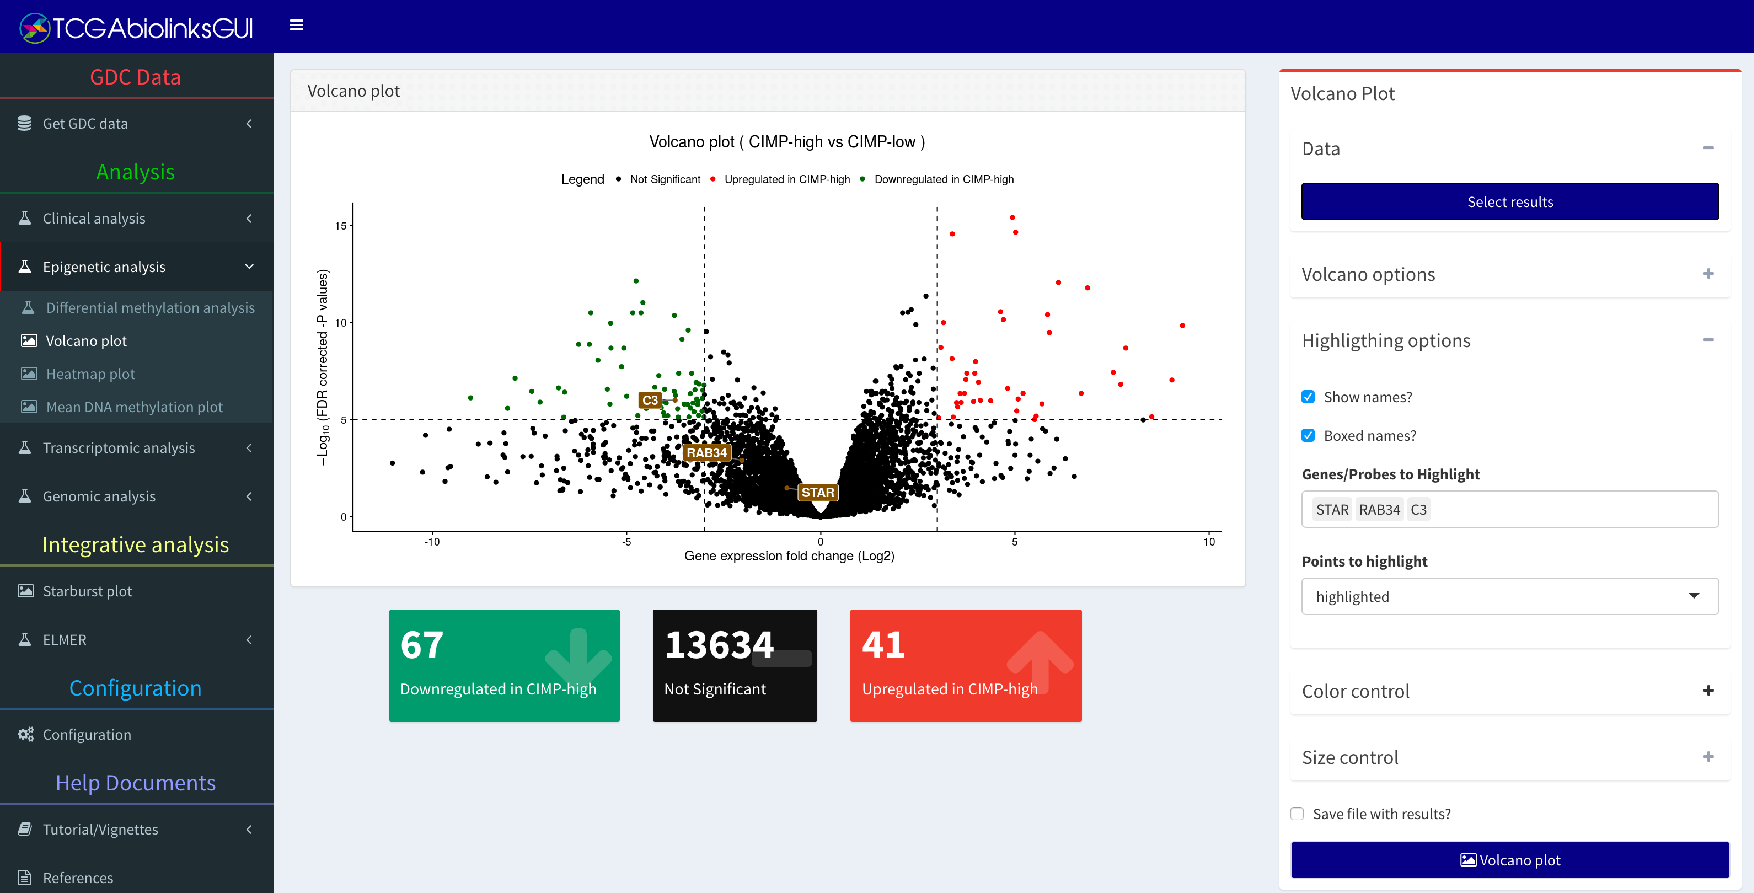
\includegraphics[width=1.0\linewidth]{images/fig1-GUI.pdf}
\caption[TCGAbiolinksGUI: The volcano plot menu]{The volcano plot menu of TCGAbiolinksGUI: The panel on the left shows the menus divided by different analyses, the panel on the right shows the controls available for the menu selected. In the center is a volcano plot window from the  analysis menu. It is possible to control the colors, to change cut-offs and to export results into a CSV document.}
\label{fig:fig1}
\end{figure}

\begin{figure}
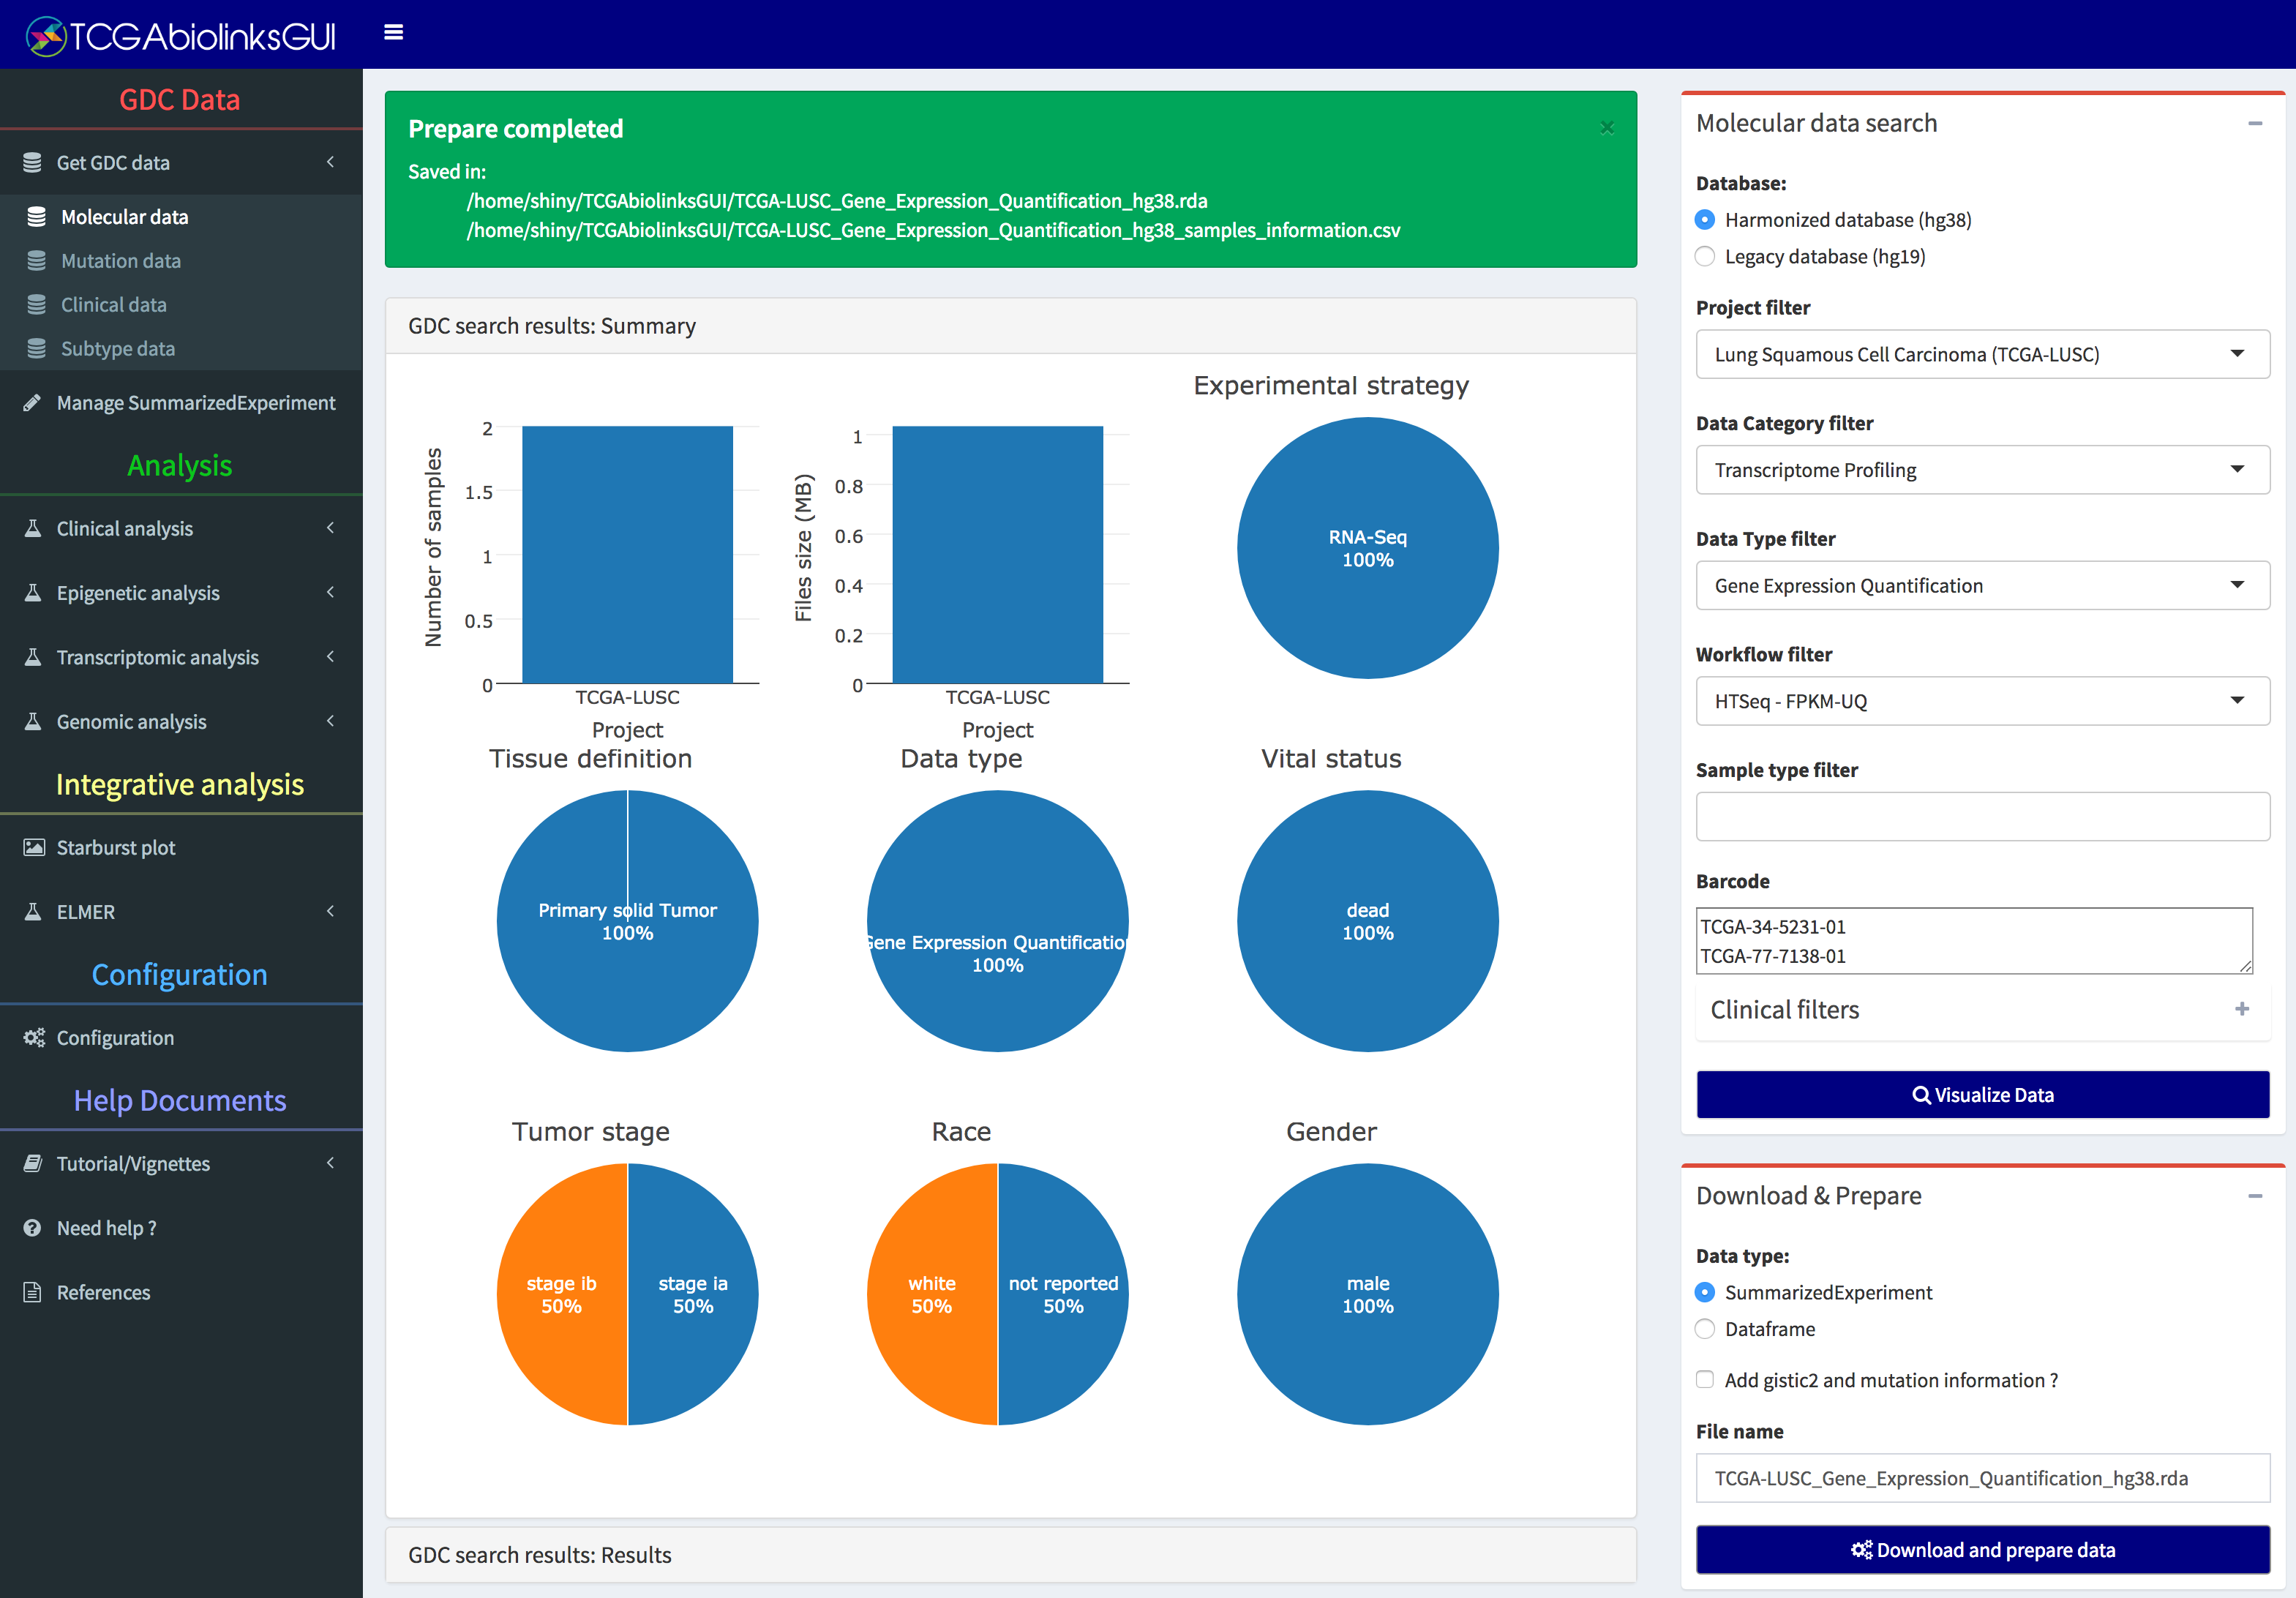
\includegraphics[width=1.0\linewidth]{images/fig2-Data_expression.png}
\caption[TCGAbiolinksGUI: Gene expression download: ]{Molecular data download: Gene expression Search, download and prepare into an R object of gene expression data for two TCGA-LUSC samples ("TCGA-34-5231-01","TCGA-77-7138-01"). The Summarized Experiment object created is saved as an RData file (TCGA-LUSC-Gene\_Expression\_Quantification\_hg38.rda). }
\label{fig:geneexp}
\end{figure}

\begin{itemize}
	\item \textbf{Data:} Provides a guided approach to search for published molecular subtype information, clinical and molecular data available in GDC. In addition, it downloads and processes the molecular data into an R object that can be used for further analysis. For raw DNA methylation data obtained in the form of Intensity Data (IDAT) files, we provide a pipeline using the R/Bioconductor minfi package (\burl{http://bioconductor.org/packages/minfi/}) to process the data for downstream analysis \cite{aryee2014minfi} performing a background and dye-bias correction with the \href{https://www.bioconductor.org/help/course-materials/2015/BioC2015/methylation450k.html\#preprocessnoob}{preprocessnoob} function followed by a detection P-value quality masking (sample-specific) \cite{morris2015analysis} and probes overlapping repeats or single nucleotide polymorphisms masking (non-sample specific) \cite{zhou2016comprehensive} (Figure \ref{fig:idat}).
	\item \textbf{Clinical analysis:} Performs survival analysis to quantify and test survival differences between two or more groups of patients and draws survival curves with the 'number at risk' table, the cumulative number of events table and the cumulative number of censored subjects table using the R/CRAN package survminer \cite{survminer}.
	\item \textbf{Epigenetic analysis:} Performs a Differentially methylated regions (DMR) analysis, visualizes the results through both volcano and heatmap plots, and visualizes the mean DNA methylation level by groups or subtypes. For certain tumor types like Glioma, we have added a function to classify non TCGA derived DNA methylation data into one of the 7 published epigenomic subtypes \cite{ceccarelli2016molecular} using a RandomForest trained model derived from DNA methylation signatures available at \burl{https://tcga-data.nci.nih.gov/docs/publications/lgggbm_2015/} (Figure \ref{fig:glioma}). Details of how these RandomForest were created are available in the \href{https://bioconductor.org/packages/devel/data/experiment/vignettes/TCGAbiolinksGUI.data/inst/doc/vignettes.html}{TCGAbiolinksGUI.data vignette} (\burl{http://bioconductor.org/packages/TCGAbiolinksGUI.data/}).
	\item \textbf{Transcriptomic analysis:} Performs a Differential Expression Analysis (DEA), and visualizes the results through both volcano and heatmap plots. Pathway analysis can be performed on a list of differentially expressed genes \cite{luo2013pathview}.
 	\item \textbf{Genomic analysis:} Visualize and summarize the mutations from MAF (Mutation Annotation Format) files through summary plots and oncoplots using the R/Bioconductor maftools package \cite{Gu20052016,Maftools} (Figures \ref{fig:maftools_summary} and \ref{fig:maftools_oncoplot}). % Cite complex heatmap
	\item \textbf{Integrative analysis:} Integrate the DMR and DEA results through a starburst plot. Integrate clinical and mutation data and perform Kaplan-Meier survival analysis for groups of mutated samples vs non-mutated for a given gene (Figure \ref{fig:mutation_clinical}). DNA methylation and gene expression data can be further analyzed using the R/Bioconductor ELMER package to discover functionally relevant genomic regions associated with cancer \cite{yao2015inferring, ELMER2}.
\end{itemize}


\begin{figure}
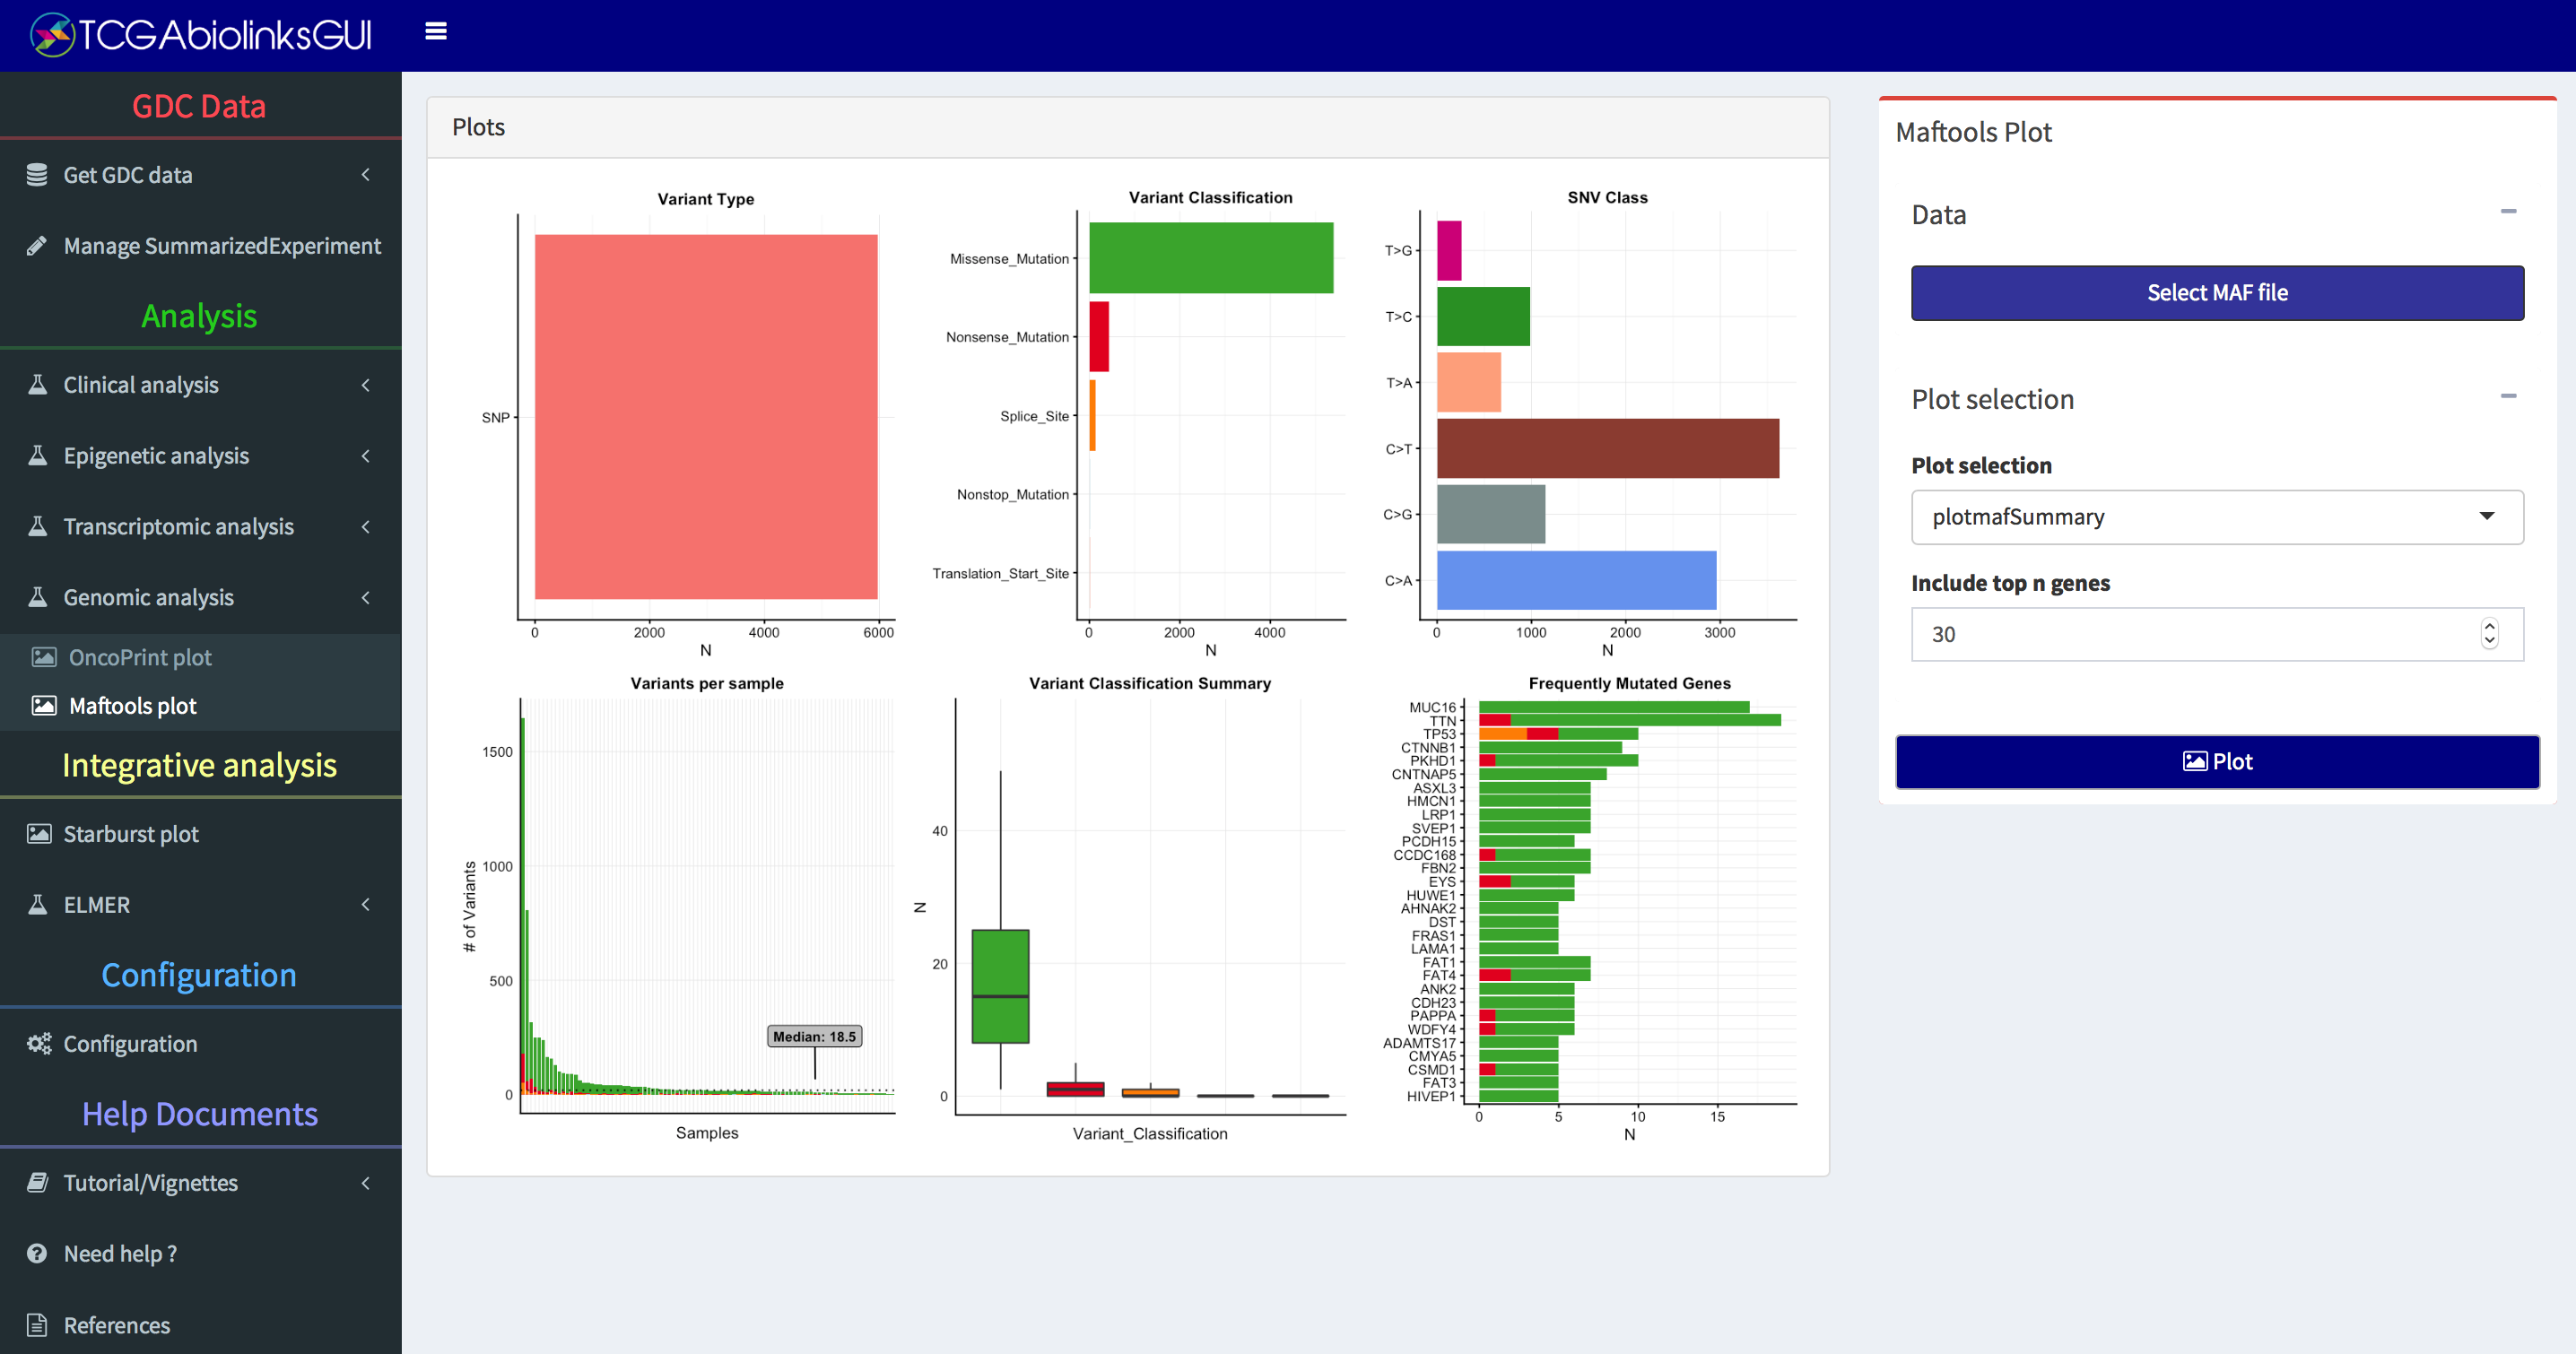
\includegraphics[width=1.0\linewidth]{images/maftools_summary.png}
\caption[TCGAbiolinksGUI: Visualizing mutation summary]{TCGAbiolinksGUI: Visualizing mutation summary. This maftools plot available thought TCGAbiolinksGUI shows a summary of the MAF file. Highlighting the most mutated genes, SNV class and variant classification distributions. }
\label{fig:maftools_summary}
\end{figure}


  \begin{figure}[h!]
  \centering
  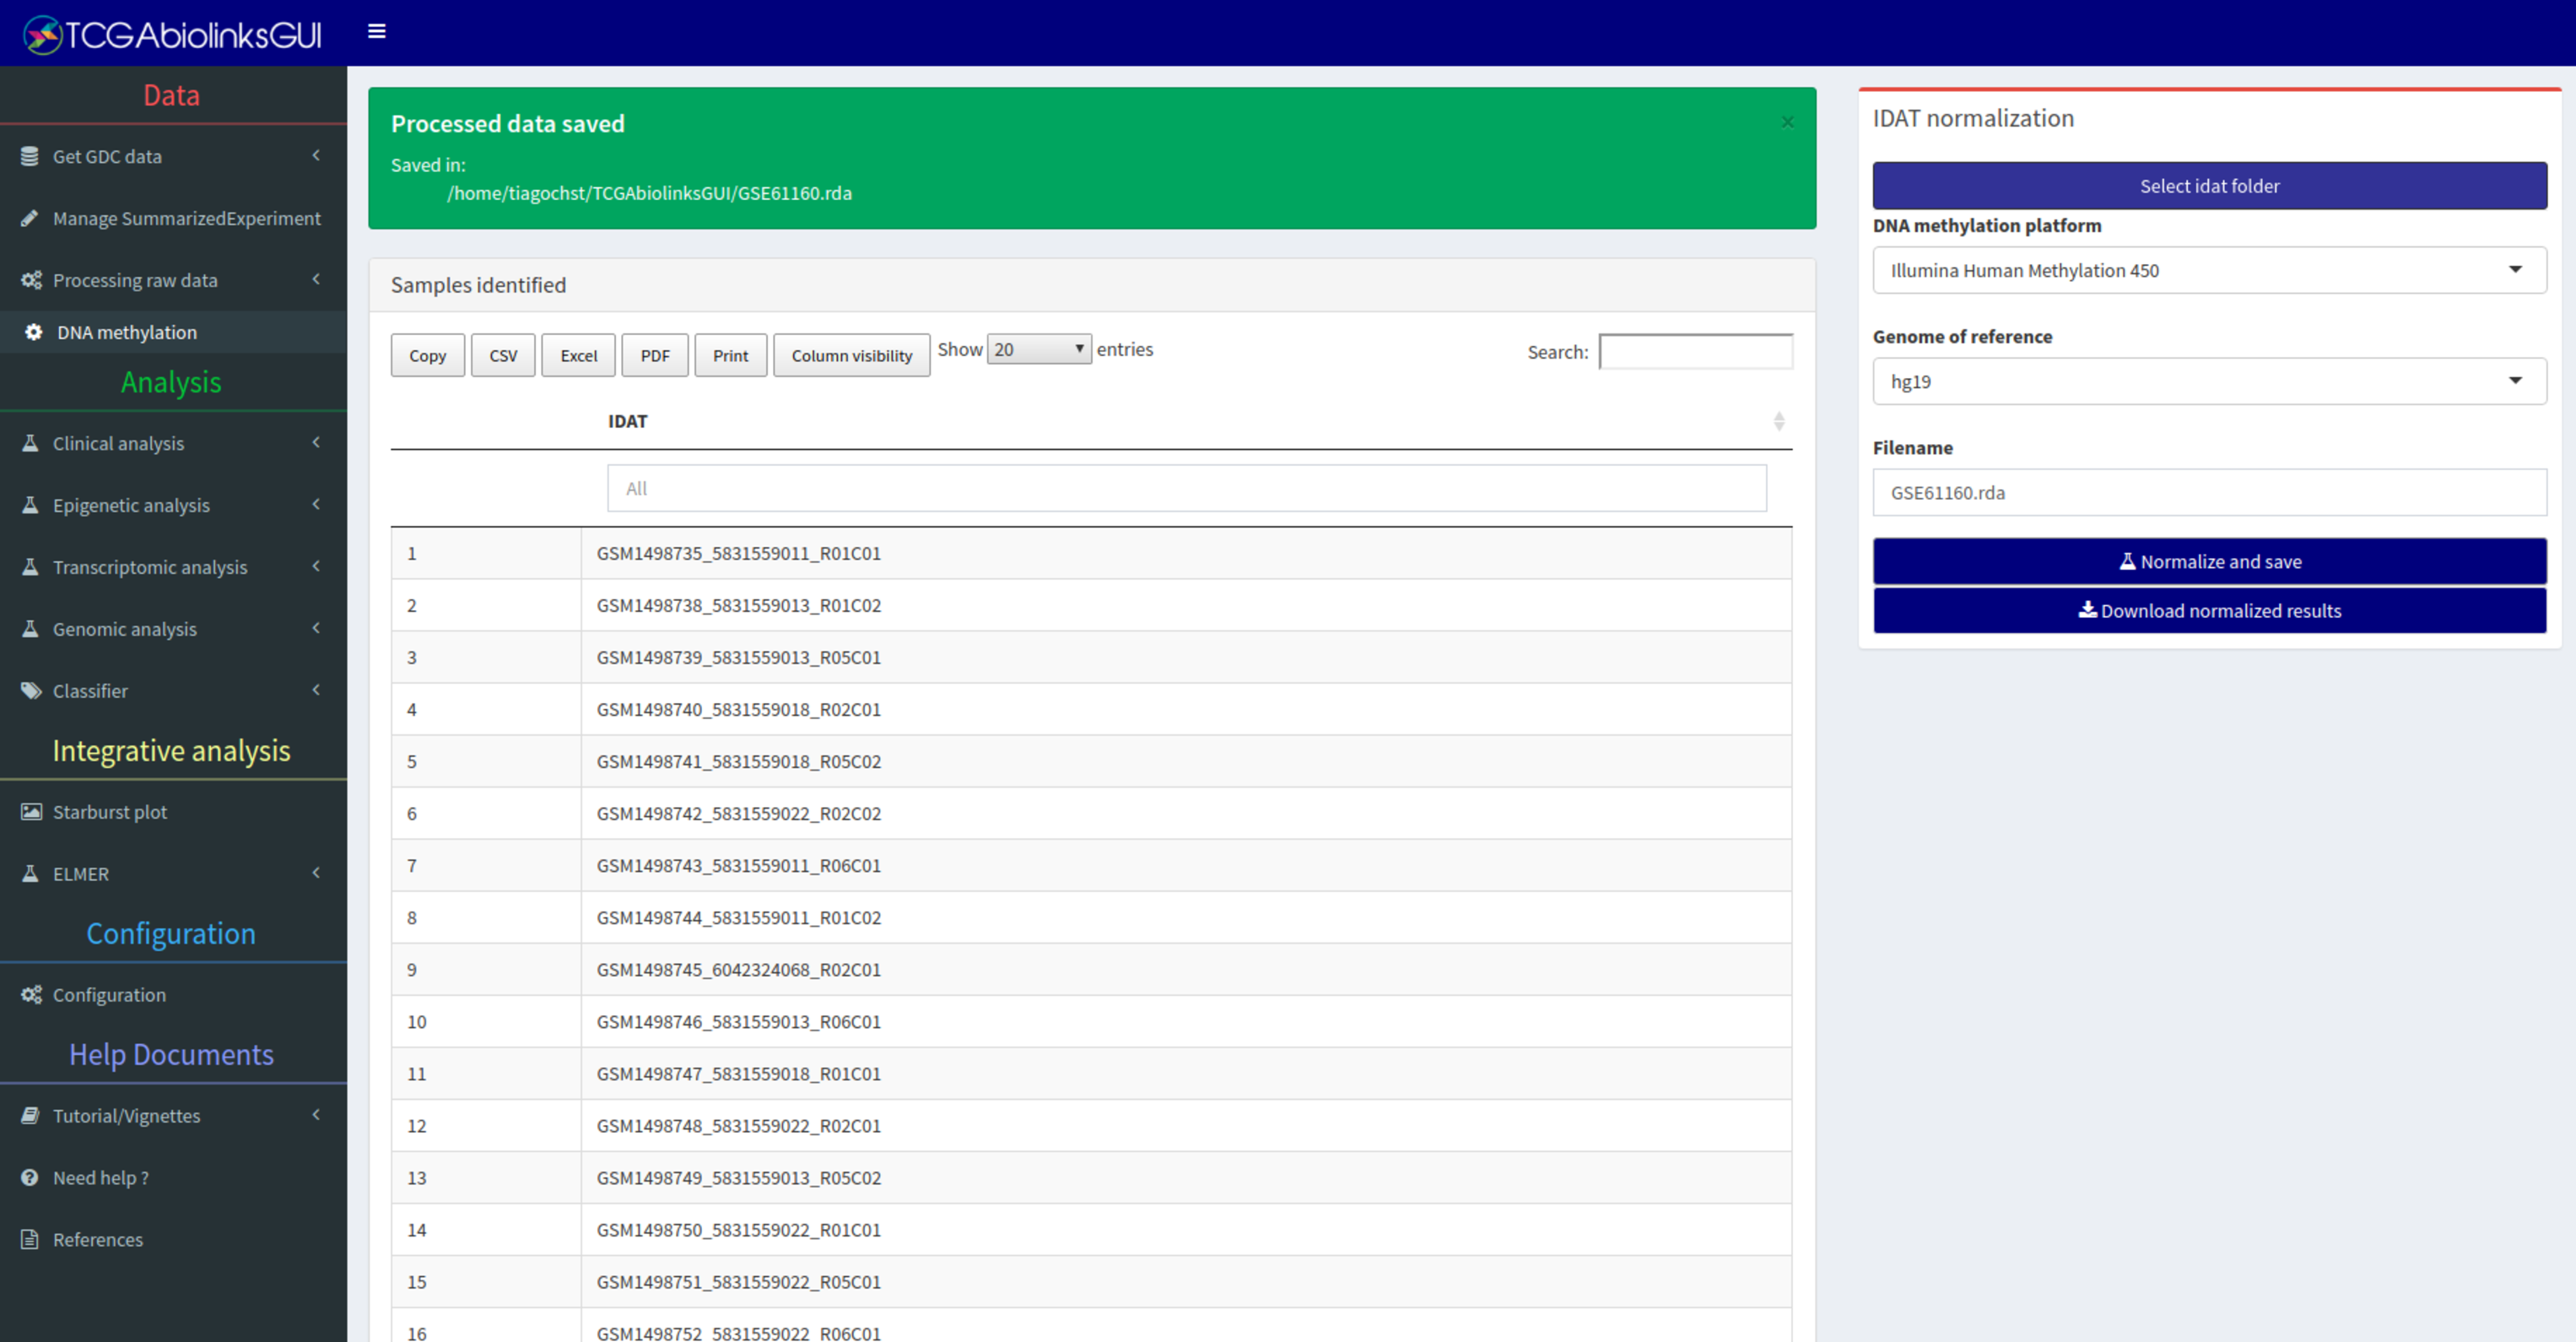
\includegraphics[width=1.0\textwidth]{images/idat.pdf}
  \caption[TCGAbiolinksGUI: IDAT normalization]{TCGAbiolinksGUI: IDAT normalization. Table shows files identified that will be processed. Data retrieved from GEO (accession GSE61160). }
  \label{fig:idat}
   \end{figure}

  \begin{figure}[h!]
  \centering
  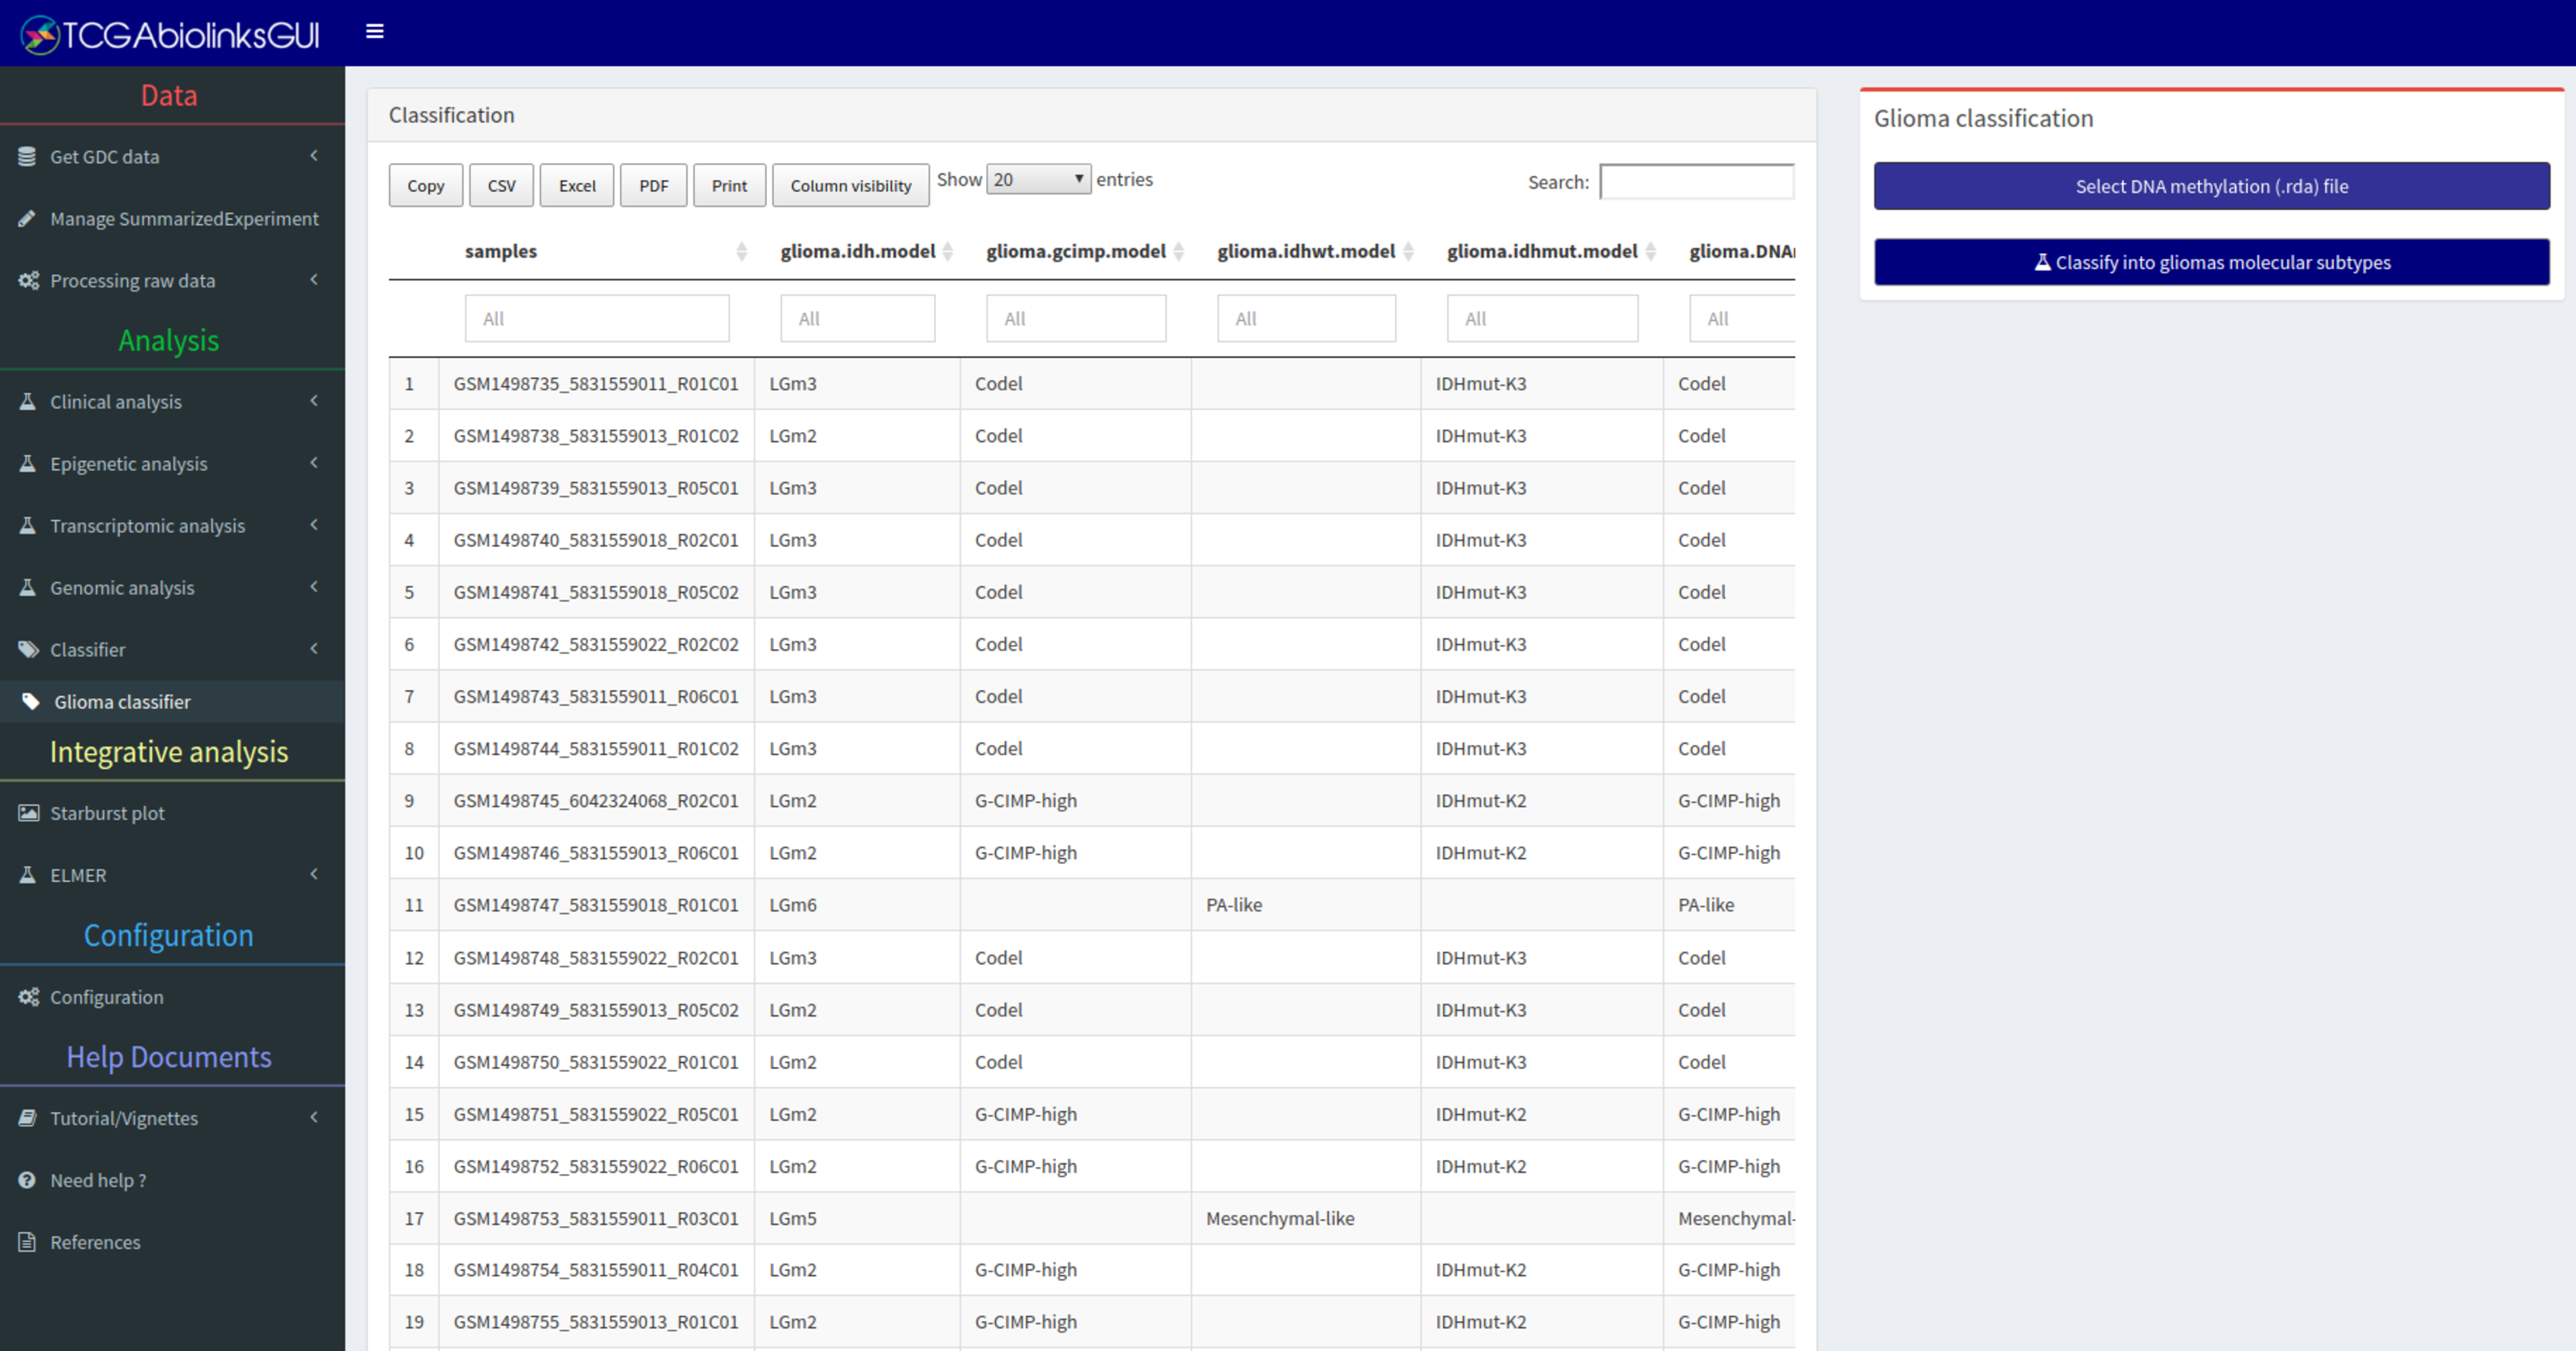
\includegraphics[width=1.0\textwidth]{images/glioma_classifier.pdf}
  \caption[TCGAbiolinksGUI: glioma classifier]{TCGAbiolinksGUI: glioma classifier. Predicting molecular subtypes based on DNA methylation using data from GEO (accession GSE61160).}
  \label{fig:glioma}
   \end{figure}

\begin{figure}
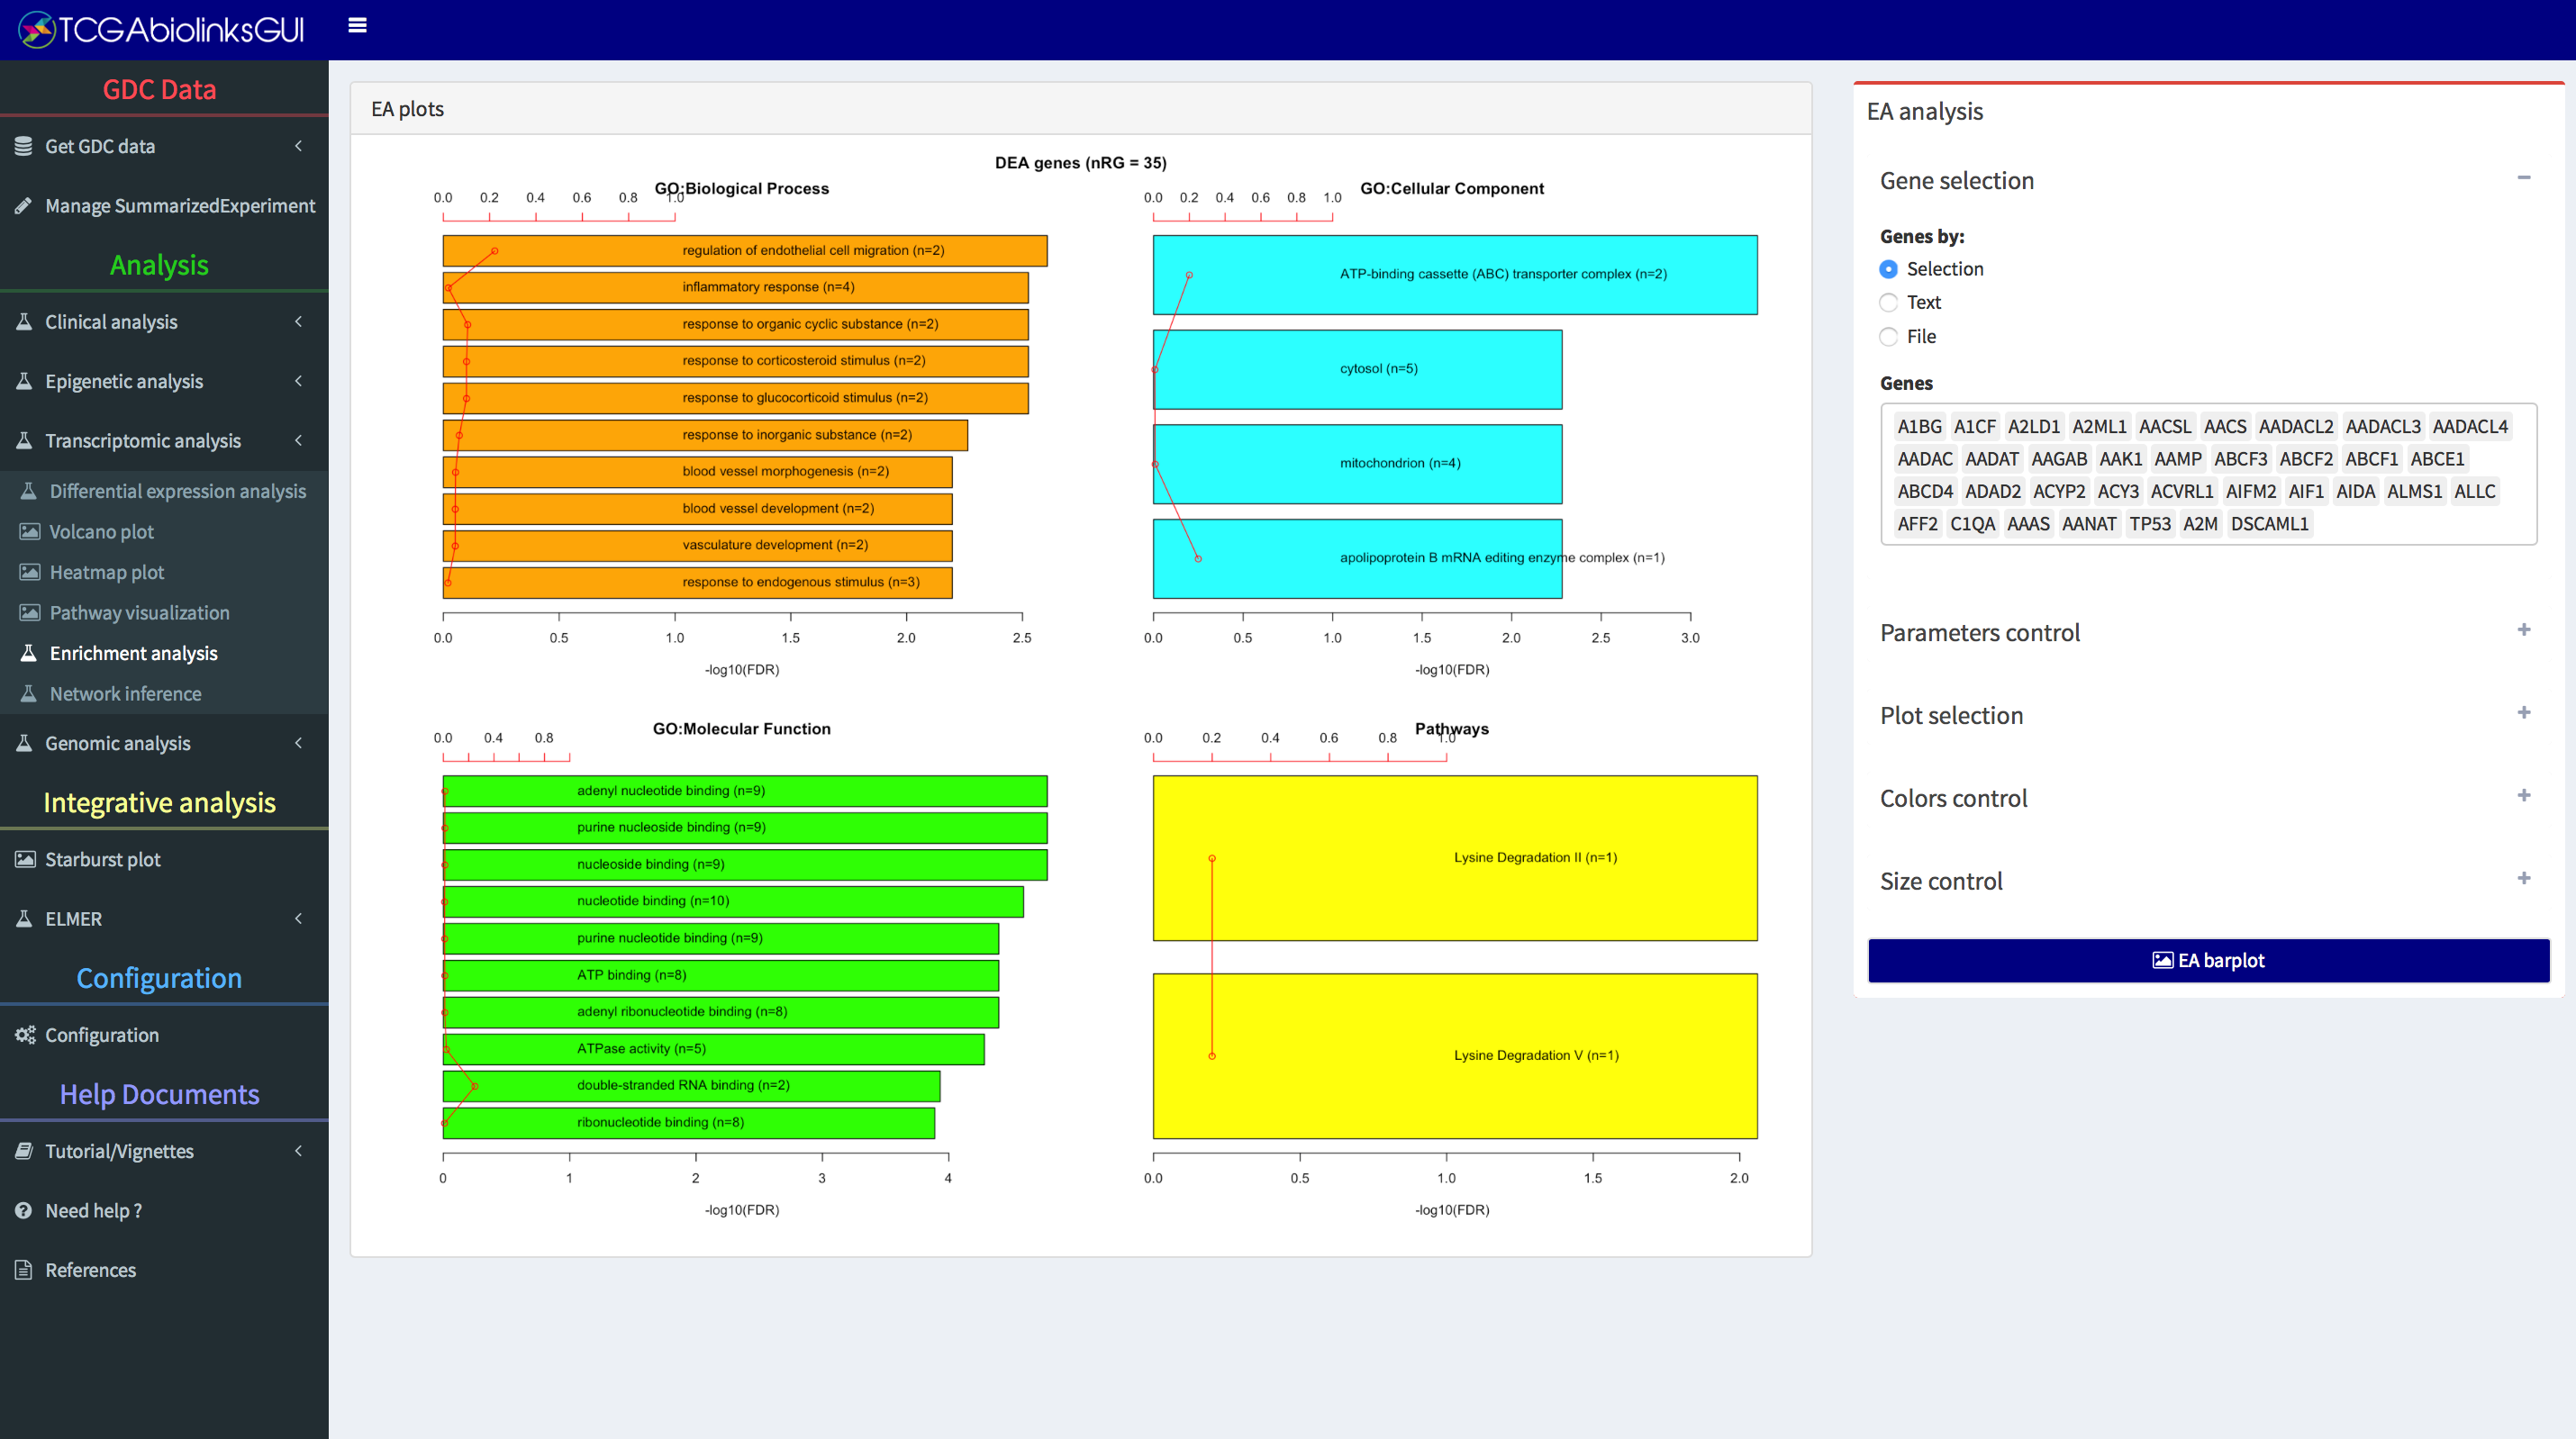
\includegraphics[width=1.0\linewidth]{images/gui_ea.png}
\caption[TCGAbiolinksGUI: Enrichement analysis of genes]{TCGAbiolinksGUI: Enrichement analysis of genes.
 TCGAbiolinks uses Gene Ontology which defines concepts/classes used to describe gene function, to perform an enrichement analysis. The plots shows  molecular function, biological process, celullar components, and pathway gene Ontology classes.
 Each barplot represents a class with the numnber of genes in the class. The width of the barplot represents the significance, and the red line represents the percentage genes inputed that is found class, for example of all genes in the biological process regulation of endothelial cell migration our 2 genes inputed represents 20\% of all genes in this process.}
\label{fig:gui_ea}
\end{figure}


\begin{figure}
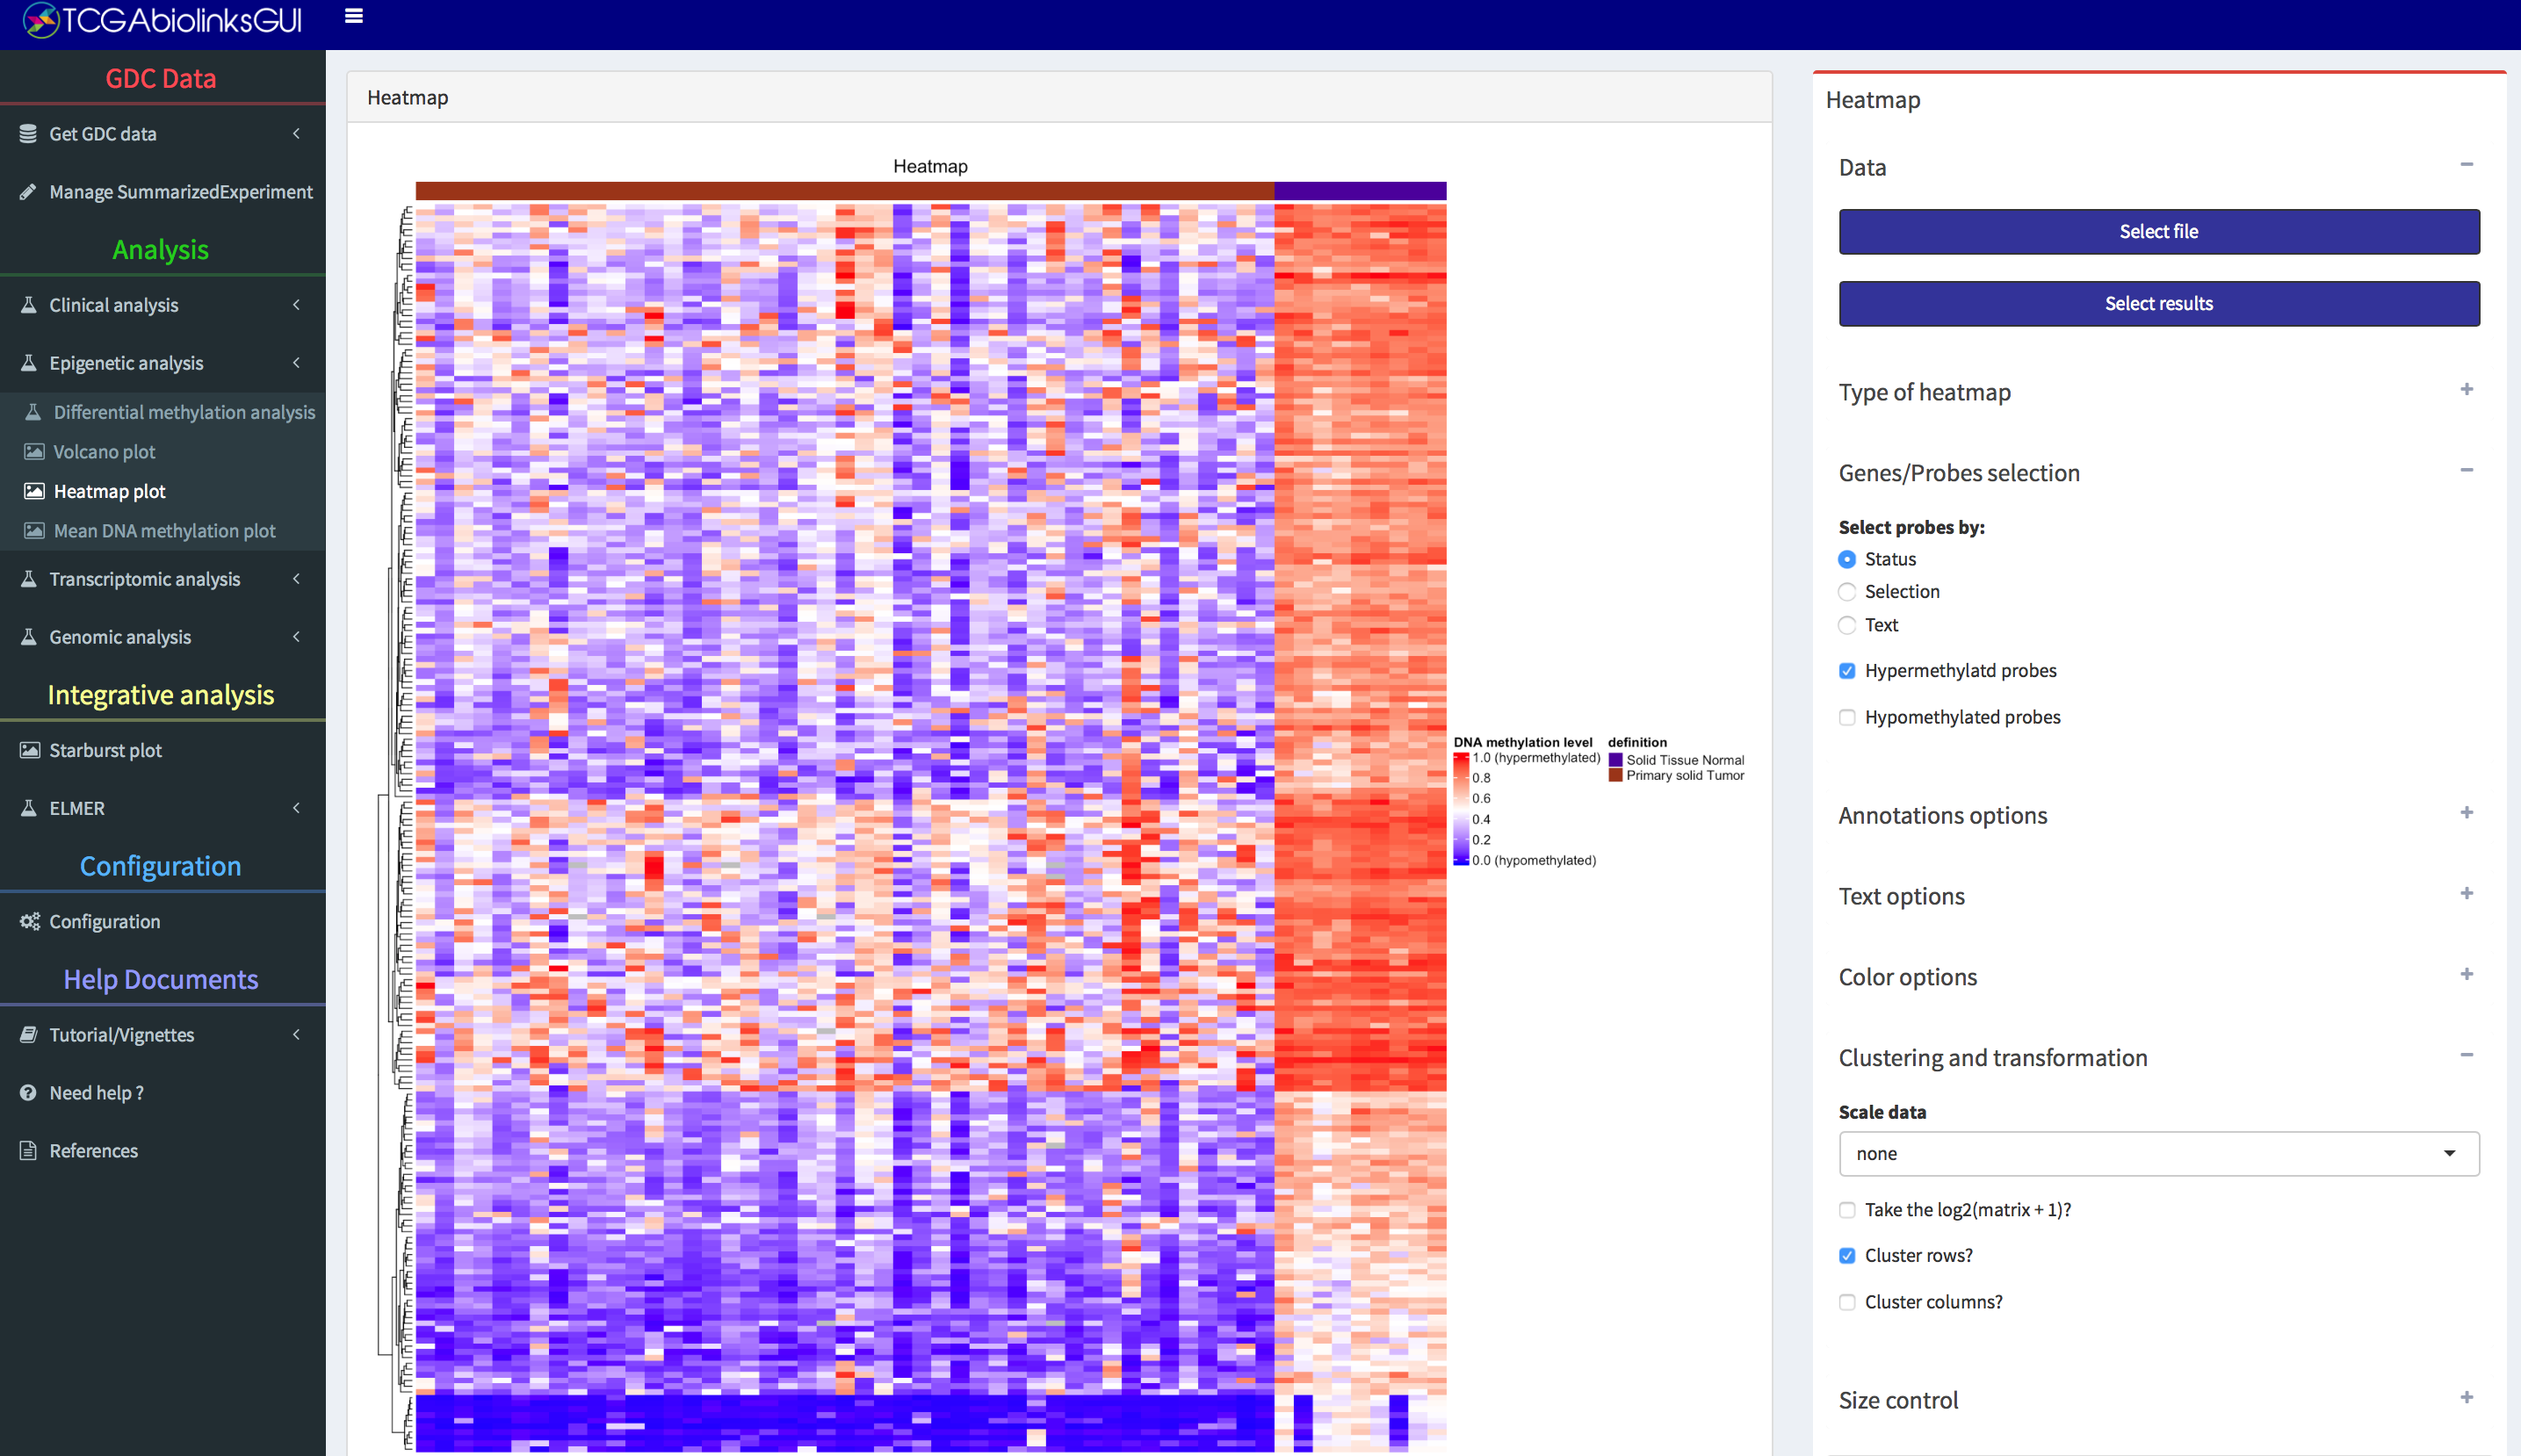
\includegraphics[width=1.0\linewidth]{images/gui_heatmap.png}
\caption[TCGAbiolinksGUI: Visualizing DMR results as heatmap]{TCGAbiolinksGUI: Visualizing DMR results as heatmap. Plot shows the DMR results: hypermethylated probes in Solid tissue normal samples compared to the Primary Solid tumor samples. Each column is a sample, while each row is a probe. Blue colors represents probes with low levels of DNA methylation and red the ones with high level. }
\label{fig:gui_heatmap}
\end{figure}

  \begin{figure}[h!]
  \centering
  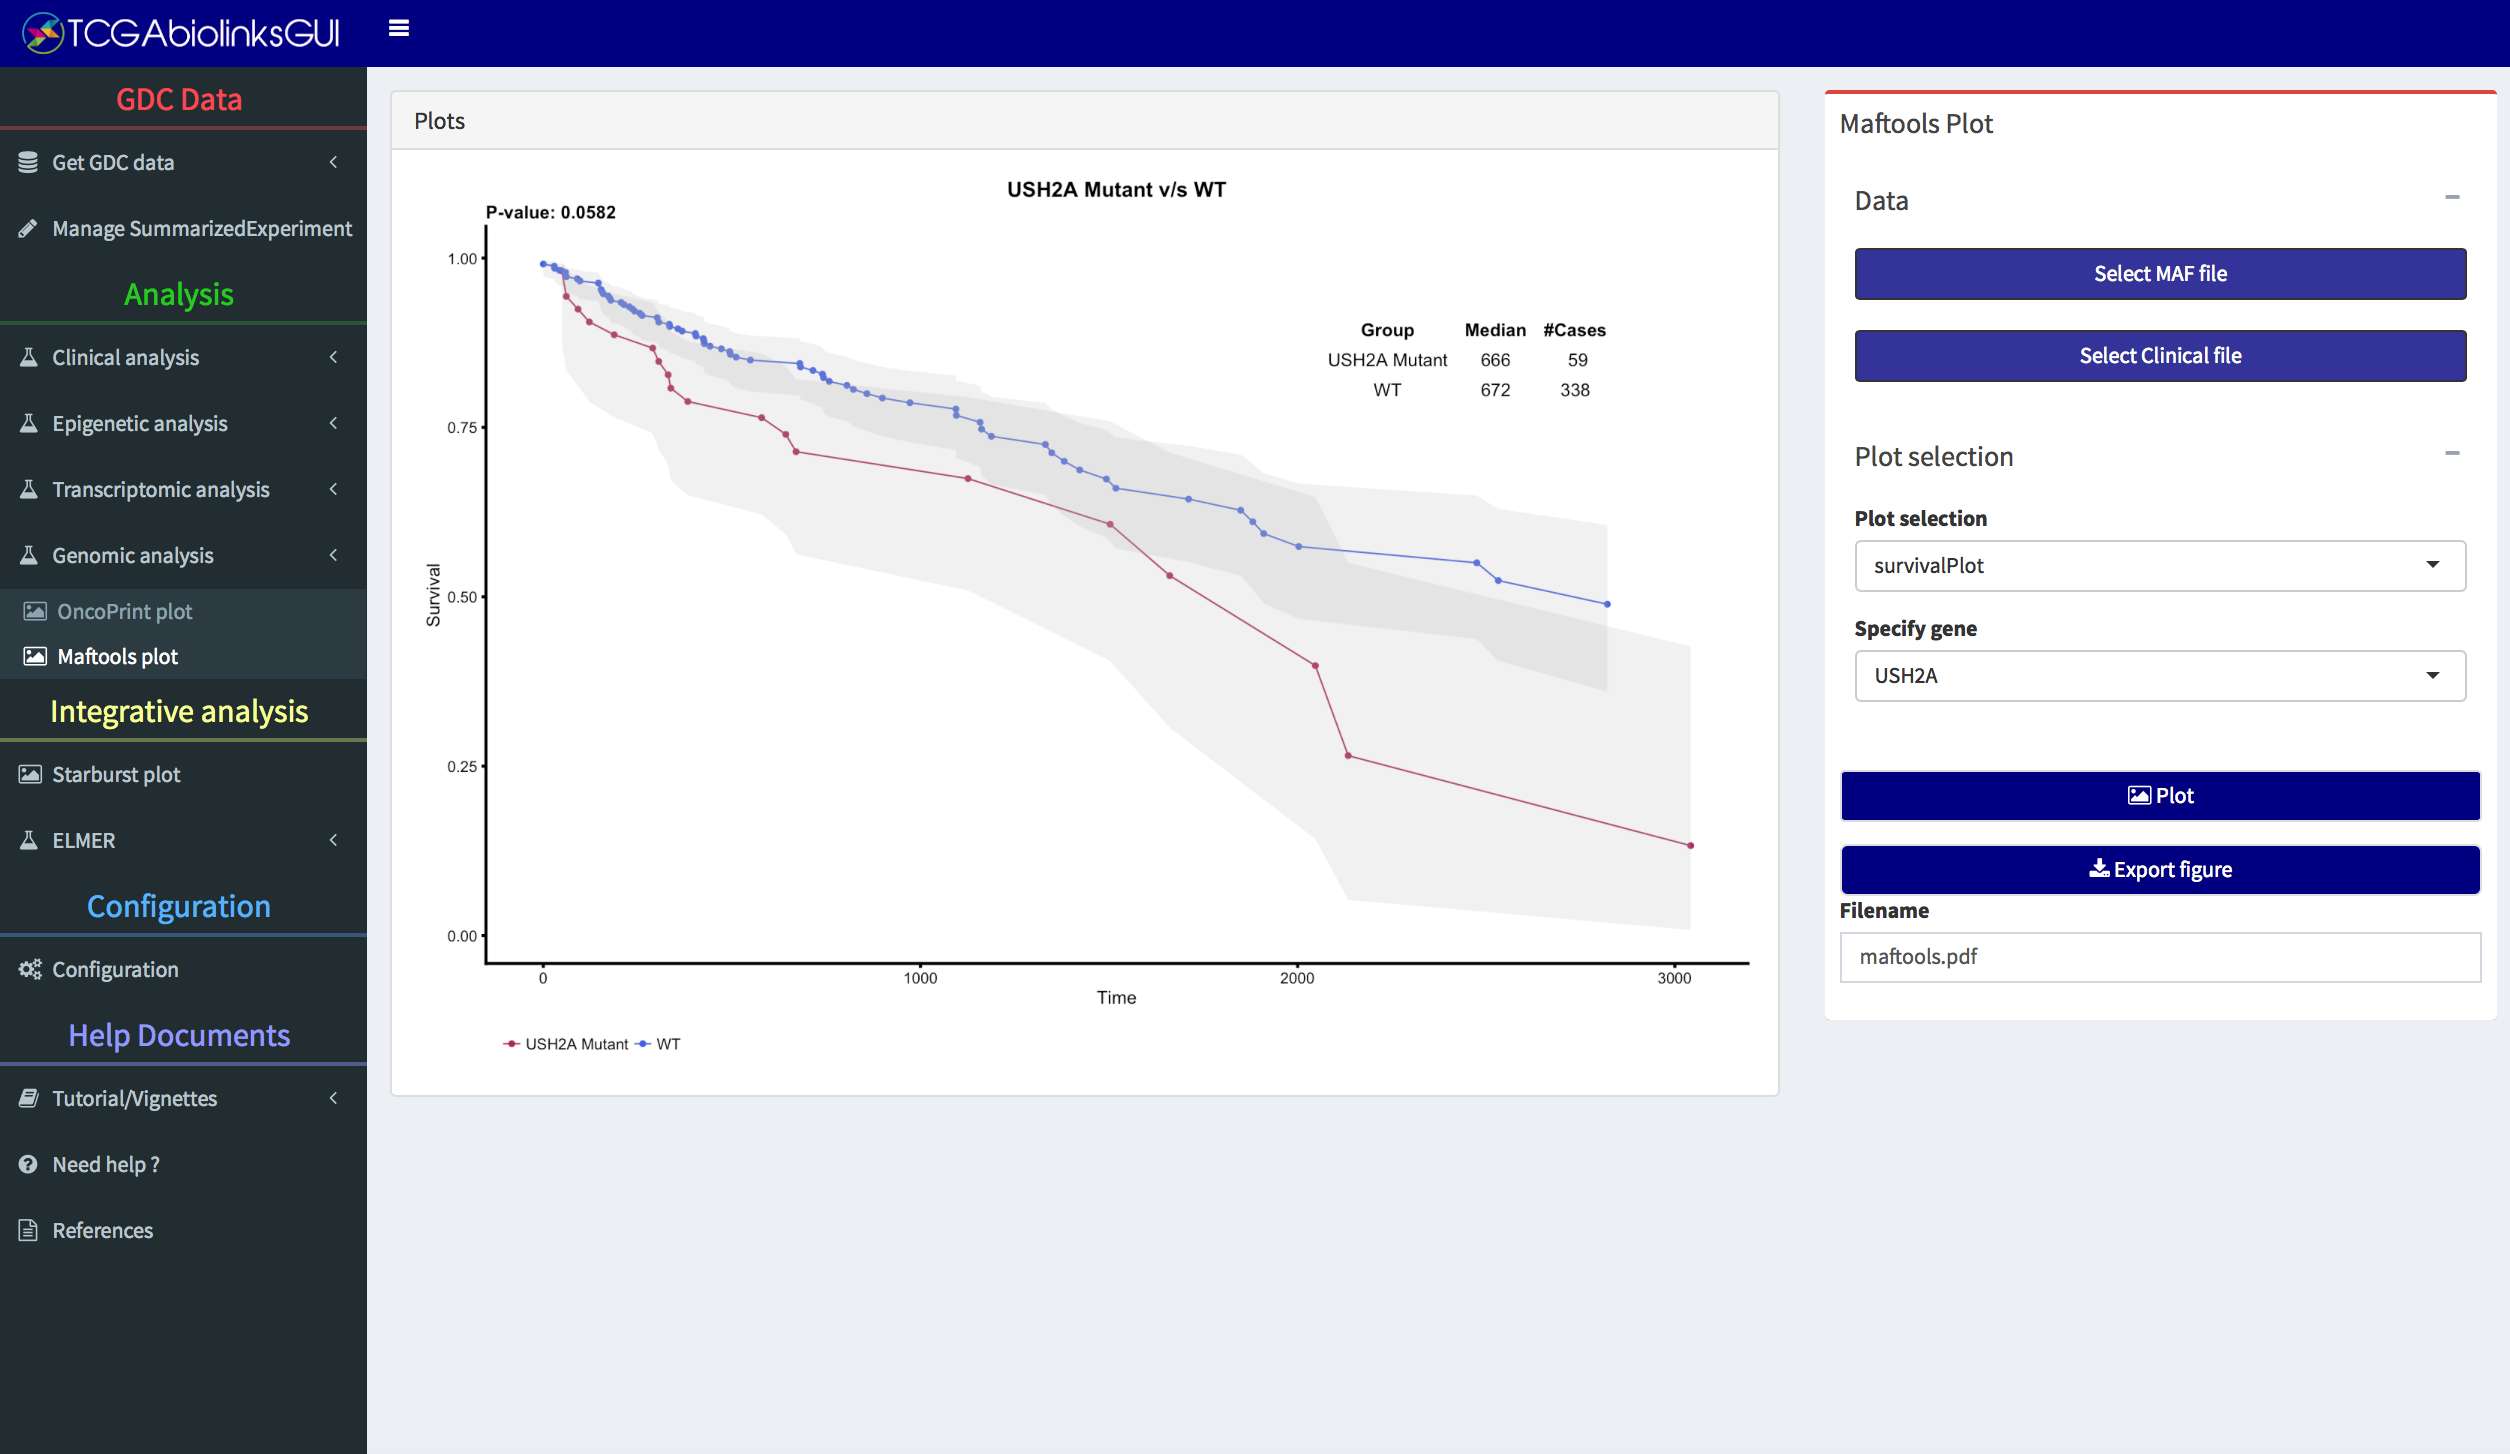
\includegraphics[width=1.0\textwidth]{images/clinical_mutation.png}
  \caption[TCGAbiolinksGUI: Integrating clinical data and mutation data]{TCGAbiolinksGUI: Integrating clinical data and mutation data. Performing Kaplan-Meier survival analysis for groups of samples with a mutation in gene USH2A vs the WT ones using the R/Bioconductor maftools package.}
  \label{fig:mutation_clinical}
   \end{figure}

\begin{figure}
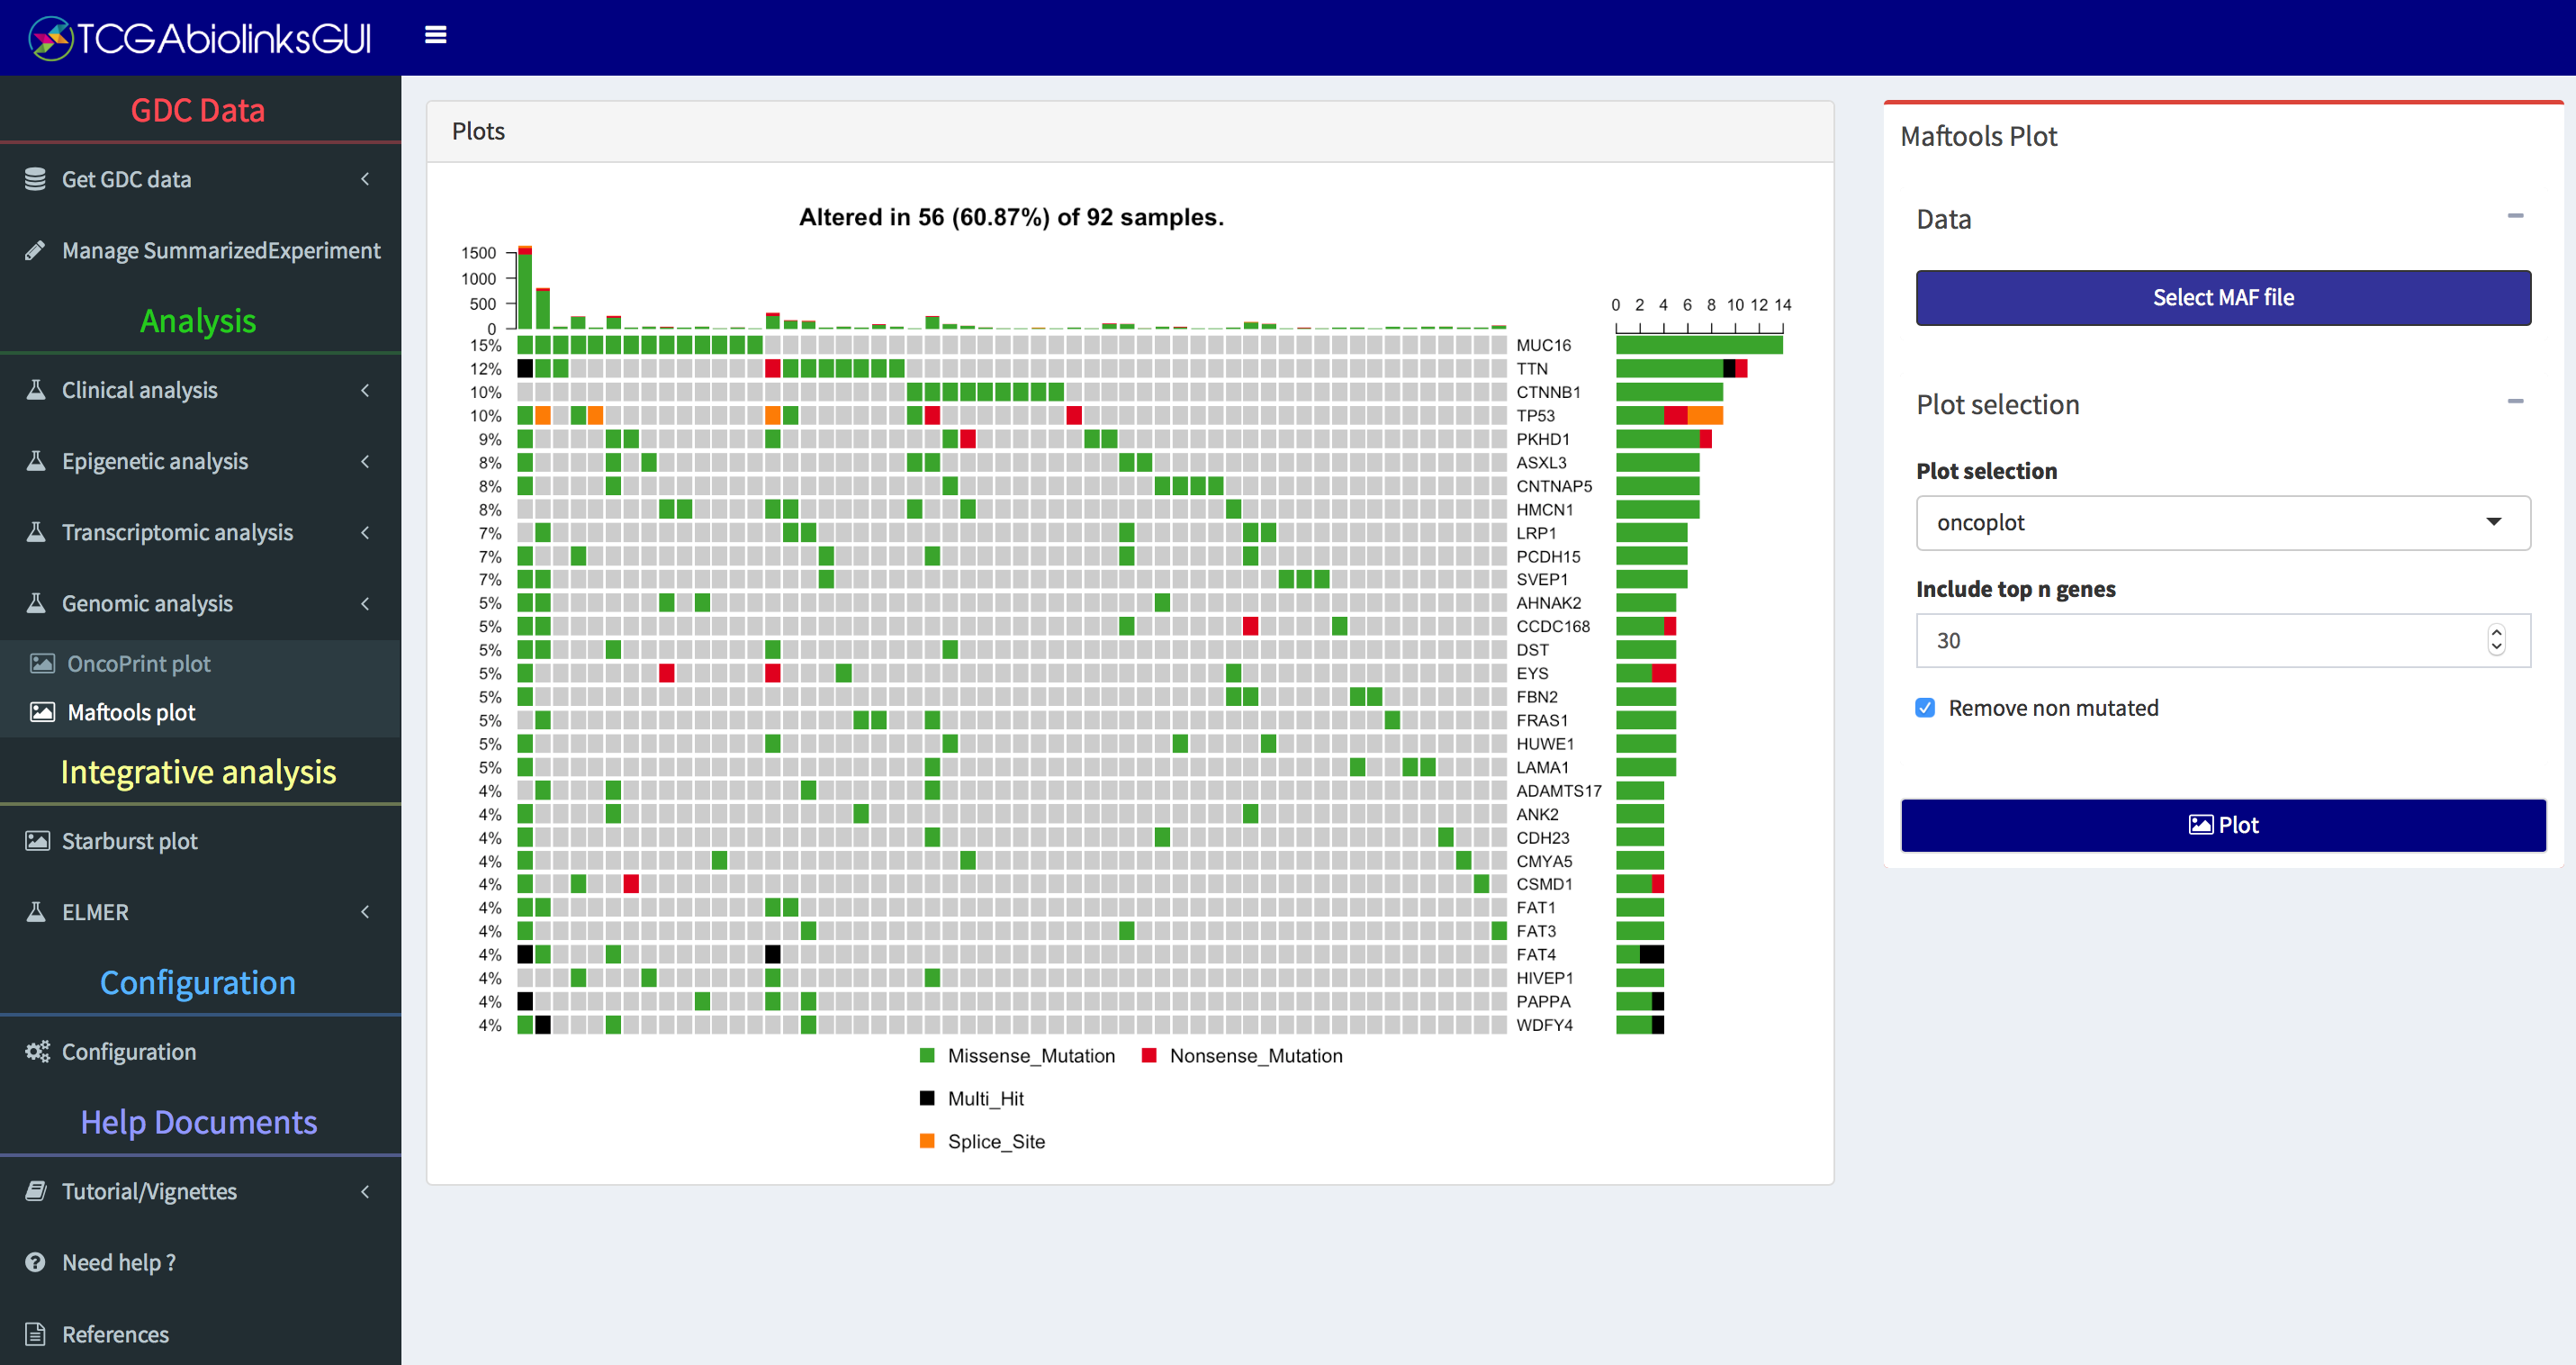
\includegraphics[width=1.0\linewidth]{images/maftools_oncoplot.png}
\caption[TCGAbiolinksGUI: Visualizing mutation as an oncoplot]{TCGAbiolinksGUI:Visualizing mutation as an oncoplot. Each column
represents a sample and each row a different gene. The top barplot has the frequency of mutations for each patient, while
the right barplot has the frequency of mutations for each gene. The plot by default is ordered by the most mutated genes.}
\label{fig:maftools_oncoplot}
\end{figure}


\begin{figure}[]
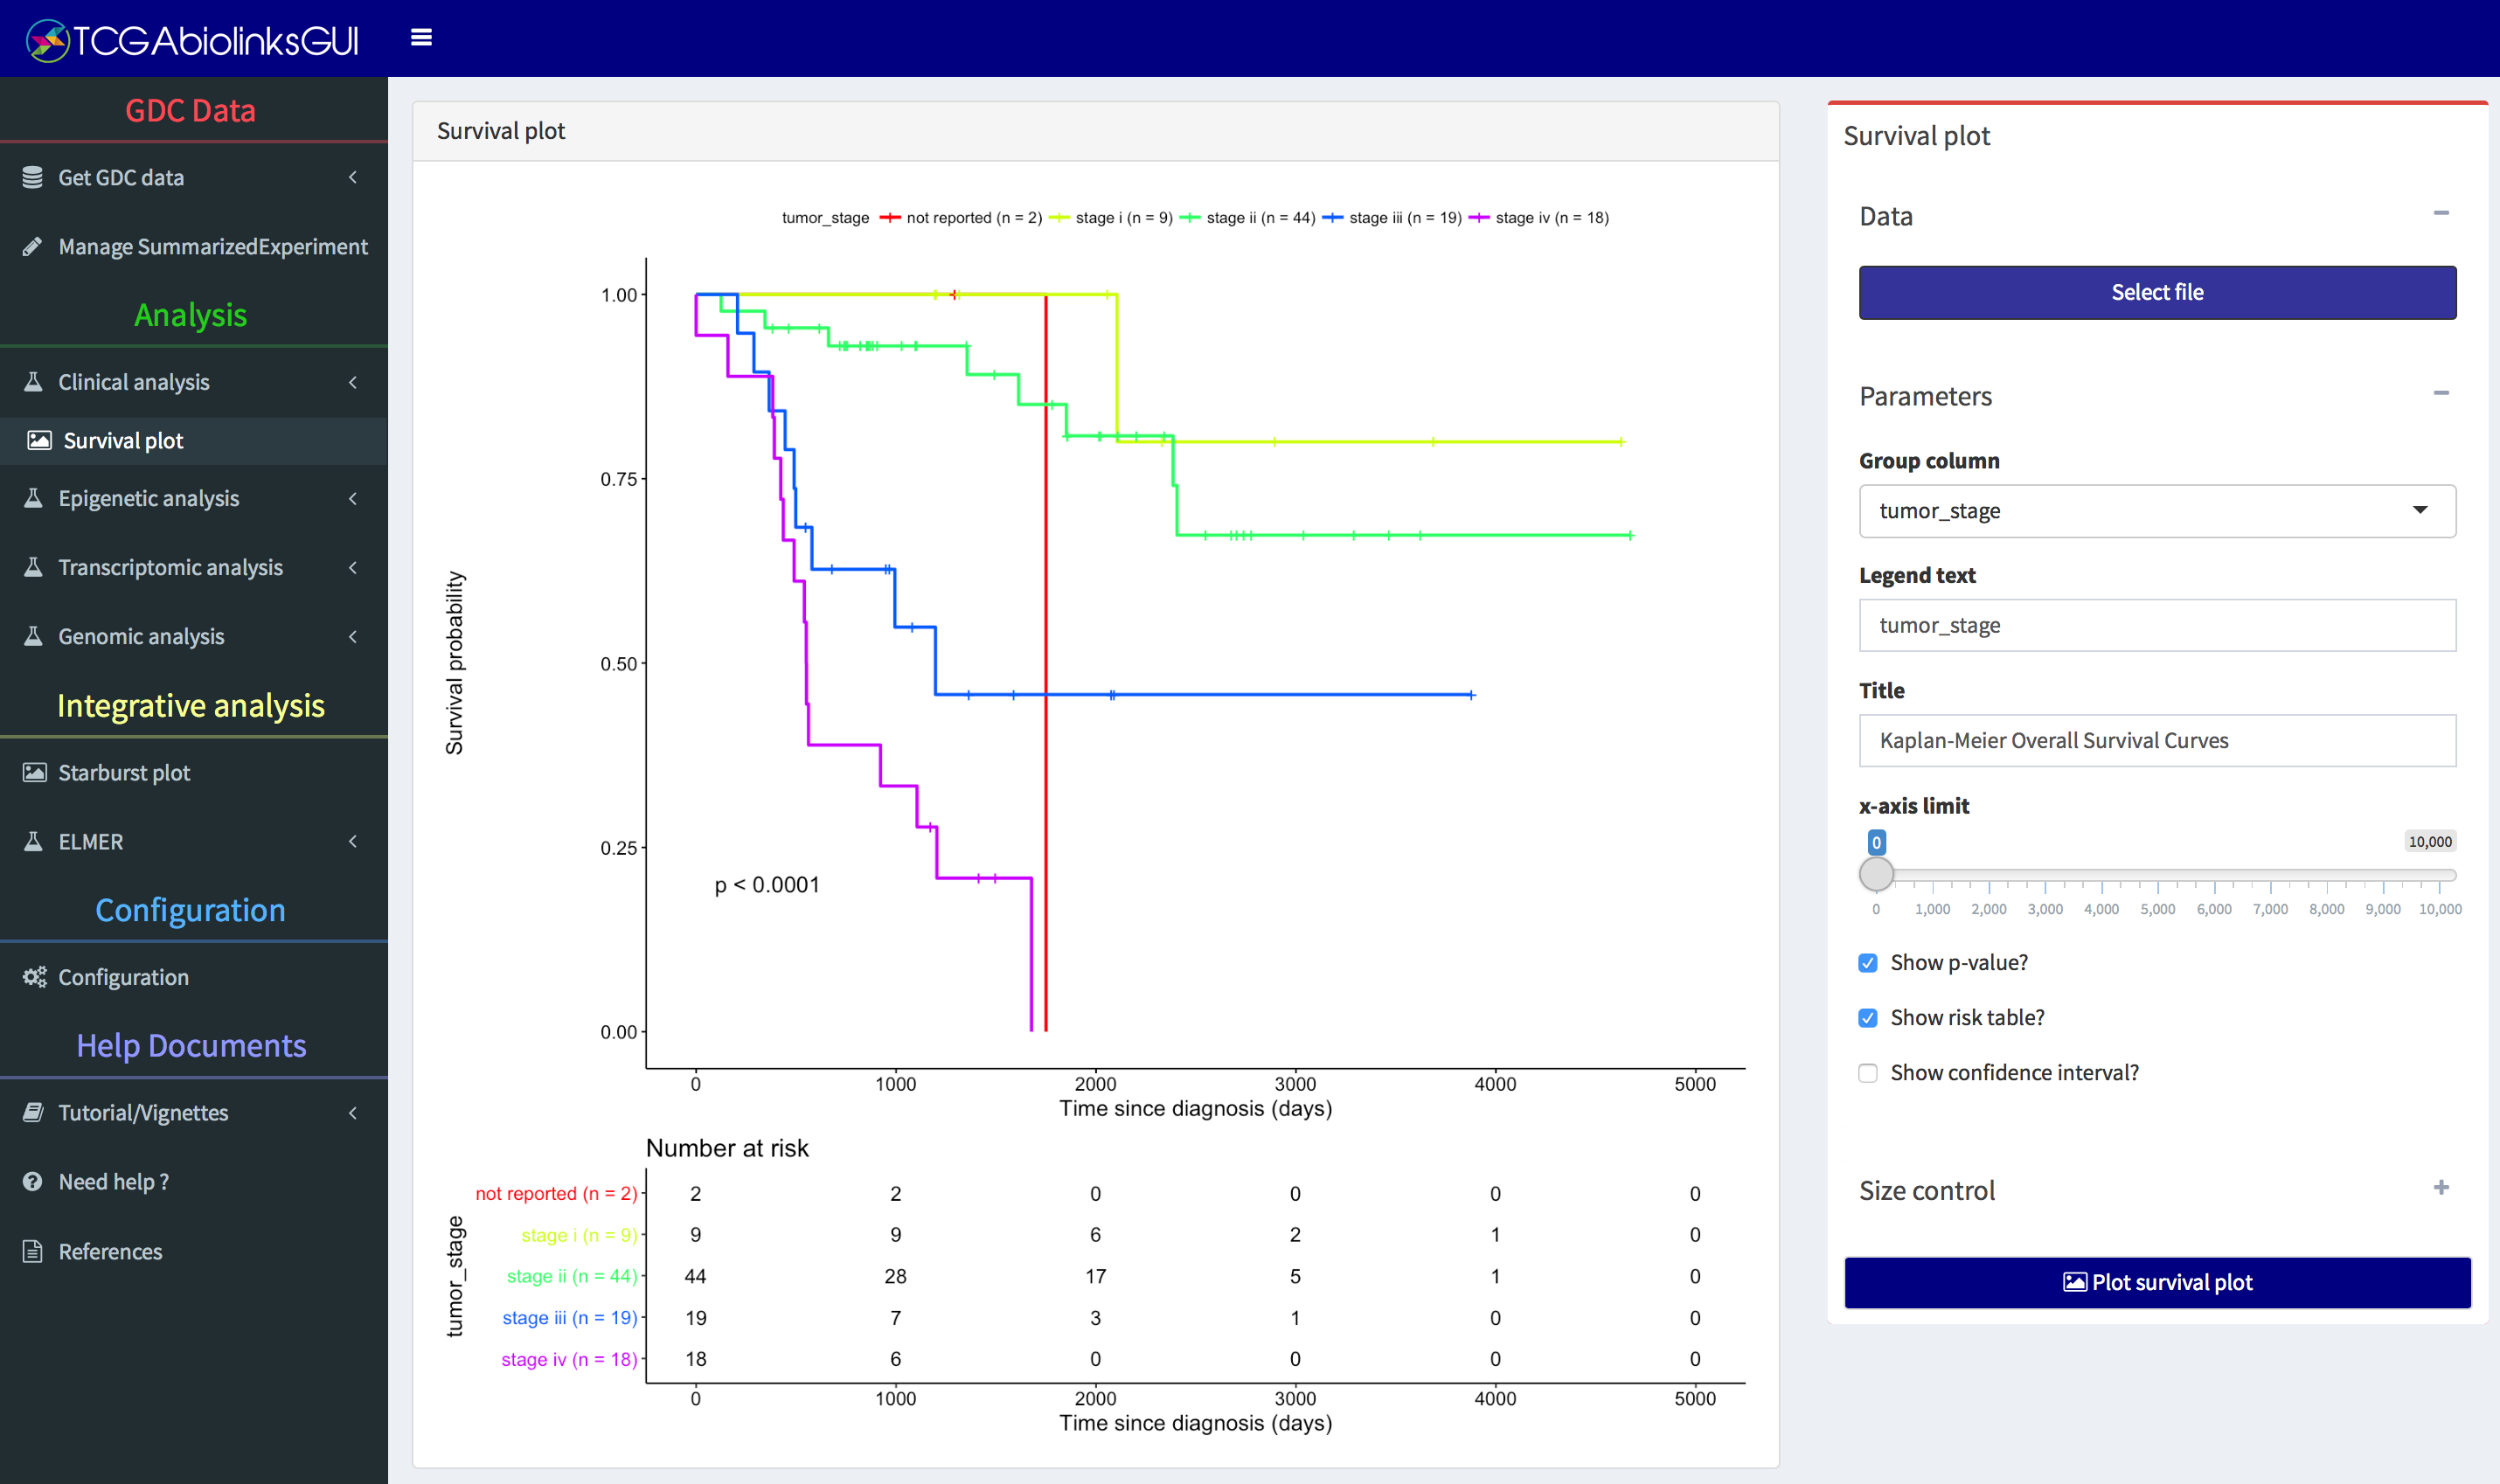
\includegraphics[width=1.0\linewidth]{images/gui_acc_survival.png}
\caption[TCGAbiolinksGUI: Survival analysis]{TCGAbiolinksGUI: Survival analysis.
The plot shows the Kaplan-Meier Overall Survival Curves for ACC (Adrenocortical carcinoma) stratified by tumor stage.
As expected, hihger levels which are more agressive have a lower survival.}
\label{fig:gui_survival}
\end{figure}

\subsection{Documentation}


We provide a guided tutorial for users via an online vignette document (\burl{http://bit.do/TCGAbiolinksDocs}) which details each step and menu function. Printable PDF (\burl{http://bit.ly/TCGAbiolinks\_PDFTutorials}) and YouTube video instructions (\burl{http://bit.ly/TCGAbiolinksGUI\_videoTutorials}) are also provided to help users utilize TCGAbiolinksGUI. A demonstration version of the tool is available at \burl{http://tcgabiolinks.fmrp.usp.br:3838/}. To help improve and expand our tool over time, users are encouraged to report and file bug reports or feature requests via our GitHub repository (\burl{https://github.com/BioinformaticsFMRP/TCGAbiolinksGUI/issues}).



\subsection{Docker container}


We recognize that one of the possible drawbacks of using our tool is the arduous process of installing R/Bioconductor environment and all of the required dependencies. To resolve this, a web version of our tool would suffice however the demand on data storage, computational processing, and multiple user access would not be justifiable and instead, we encourage users to use their own computers. However, to further simplify the usability and accessibility of our tool, we provide a Docker image file. This file is compatible with most popular operating systems and it is available online at \burl{https://hub.docker.com/r/tiagochst/tcgabiolinksgui/}. It contains the complete R/Bioconductor environment configured to use TCGAbiolinksGUI. By providing a Docker image, we anticipate users with very little knowledge of R/Bioconductor to run TCGAbiolinksGUI without the need to install associated dependencies or configure system files, common steps required to run R installations and load R/Bioconductor packages.  This image can be easily downloaded and deployed through the Kitematic tool (\burl{https://kitematic.com/}), a simple application for managing Docker containers for Mac, Linux, and Windows. A detailed documentation on how to get and use the docker image via the Kitematic application is available at
\burl{http://bit.ly/TCGAbiolinksGUI_docker}. The Docker image will be updated as regularly as TCGAbiolinksGUI thus providing several types of access for end-users interested in analyzing TCGA data from GDC.



\subsection{Comparison of alternative software}


Web tools used for cancer data analysis might be classified into two broad groups.
The first group only provides an interface to existing software analysis tools.
The Galaxy project (\burl{https://galaxyproject.org/}), which is an open, web-based platform for accessible, reproducible, and transparent computational biomedical research, is an example of such a tool that belongs to this group.
The other group is composed of exploratory tools mainly focused on the visualization of processed data and pre-computed results. The cBioPortal project \cite{gao2013integrative,cerami2012cbio}, by providing several visualizations for mining the TCGA data, is an example of a tool that falls within this classification.

If one were to correctly classify TCGAbiolinksGUI, it would belong to the first group. Compared to the Galaxy project, TCGAbiolinksGUI offers an open platform which improves the accessibility of R/Bioconductor packages, allowing users an advantage to integrate their features with existing Bioconductor packages without the need to go beyond the R/Shiny frameworks as a common feature from the Galaxy project, which requires the interface elements to be structured through XML files \cite{10.12688/f1000research.9821.1}.
In addition, outside of the R/Bioconductor environment requires more software dependencies which make the process to install Galaxy + R/Bioconductor packages laborious and cumbersome, something most non-bioinformaticians are eager to contend with.
Compared to cBioPortal, TCGAbiolinksGUI not only provides users with access to raw and processed data, but TCGAbiolinksGUI allows users to perform a deep integrative analysis which is not currently available in cBioPortal.  For example, if a user is interested in defining differentially expressed genes or DNA methylation events between two populations of tumors (i.e. FOXA1 mutants and wildtypes), cBioPortal would only allow users access to the samples data and expect the users to download and analyze within their own favorite tool thus limiting many users from implementing this type of analysis. TCGAbiolinksGUI takes the groups of samples and can define a list of differentially expressed genes, pathway analysis, and even survival analysis all within one tool without the need to perform any further bioinformatics integration.
